\chapter{Mapas de Calor da Campanha de Robustez}
\label{ap:robustez}

Os mapas a seguir apresentam, para cada configuração de algoritmo e parâmetros, os valores consolidados nos atrasos de gargalo de 10 ms, 50 ms e 100 ms. As linhas identificam o algoritmo e, no caso do CUBIC-RTT, os valores de $\alpha$ e $\gamma$.

\section{Cenário bw1\_f4}

\begin{figure}[p]
\centering
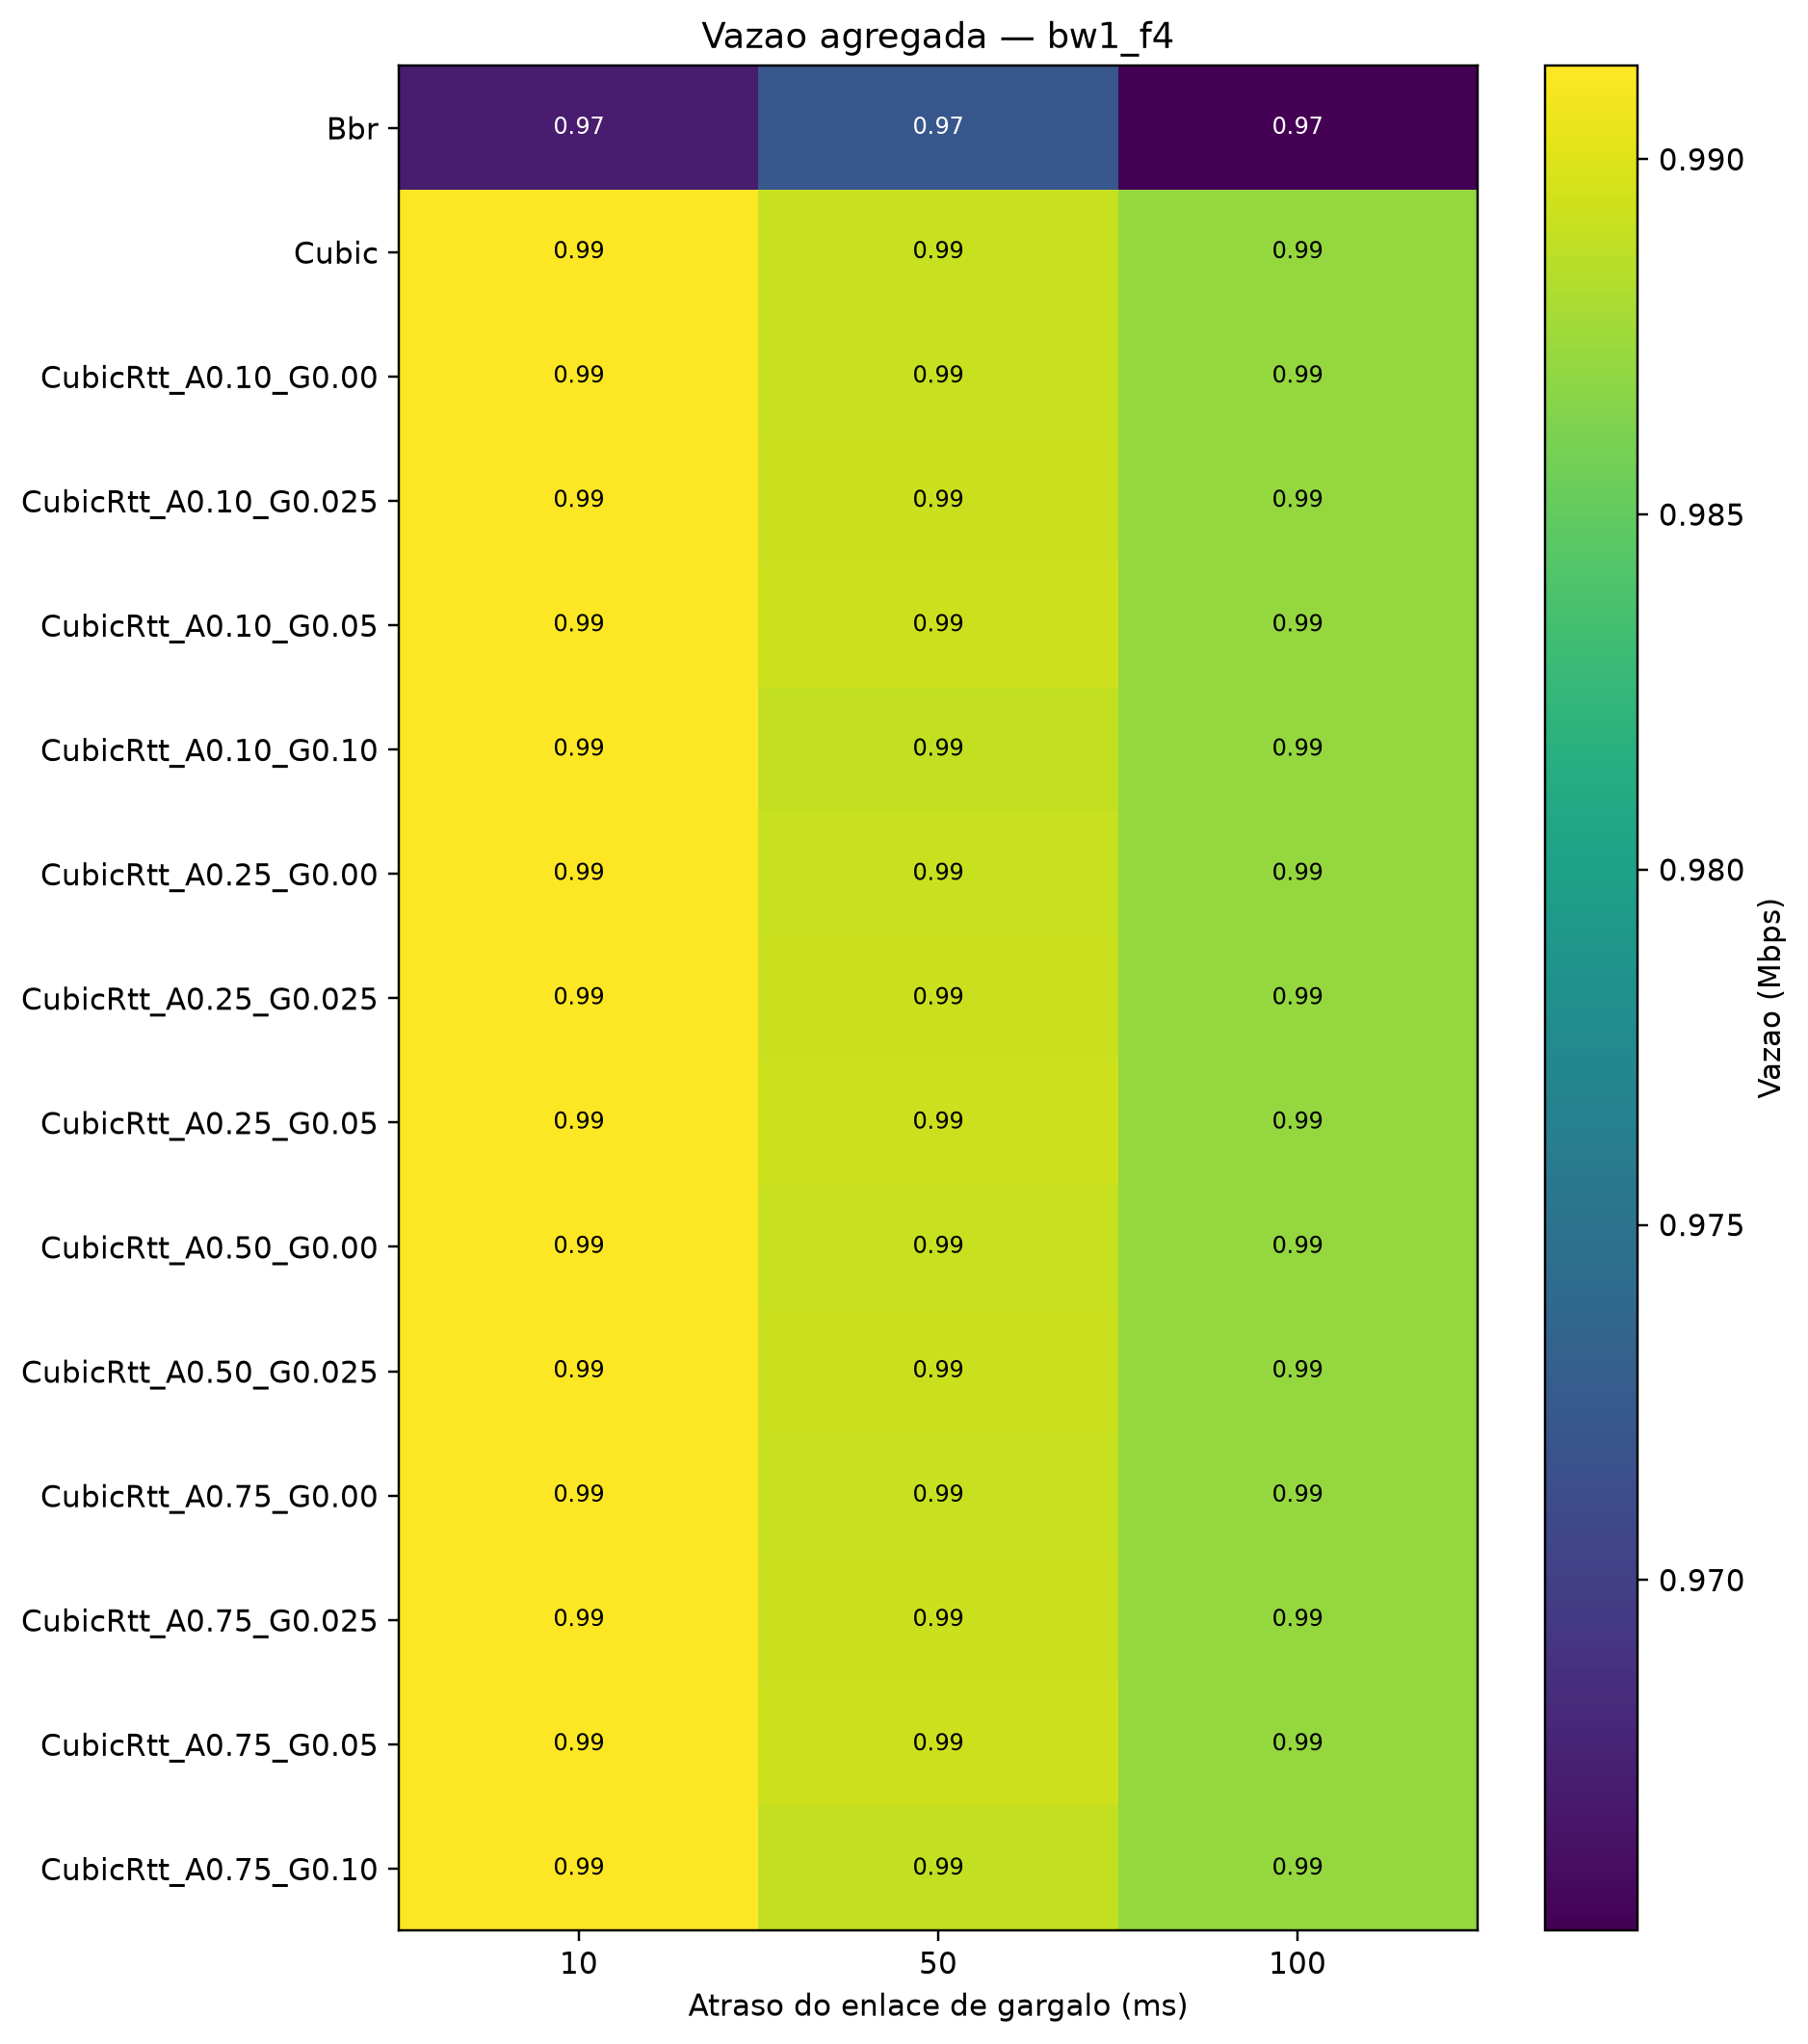
\includegraphics[width=0.88\textwidth]{bw1_f4_throughput_mbps.png}
\caption{Vazão agregada no cenário \texttt{bw1\_f4}.}
\label{fig:bw1-throughput}
\end{figure}

\begin{figure}[p]
\centering
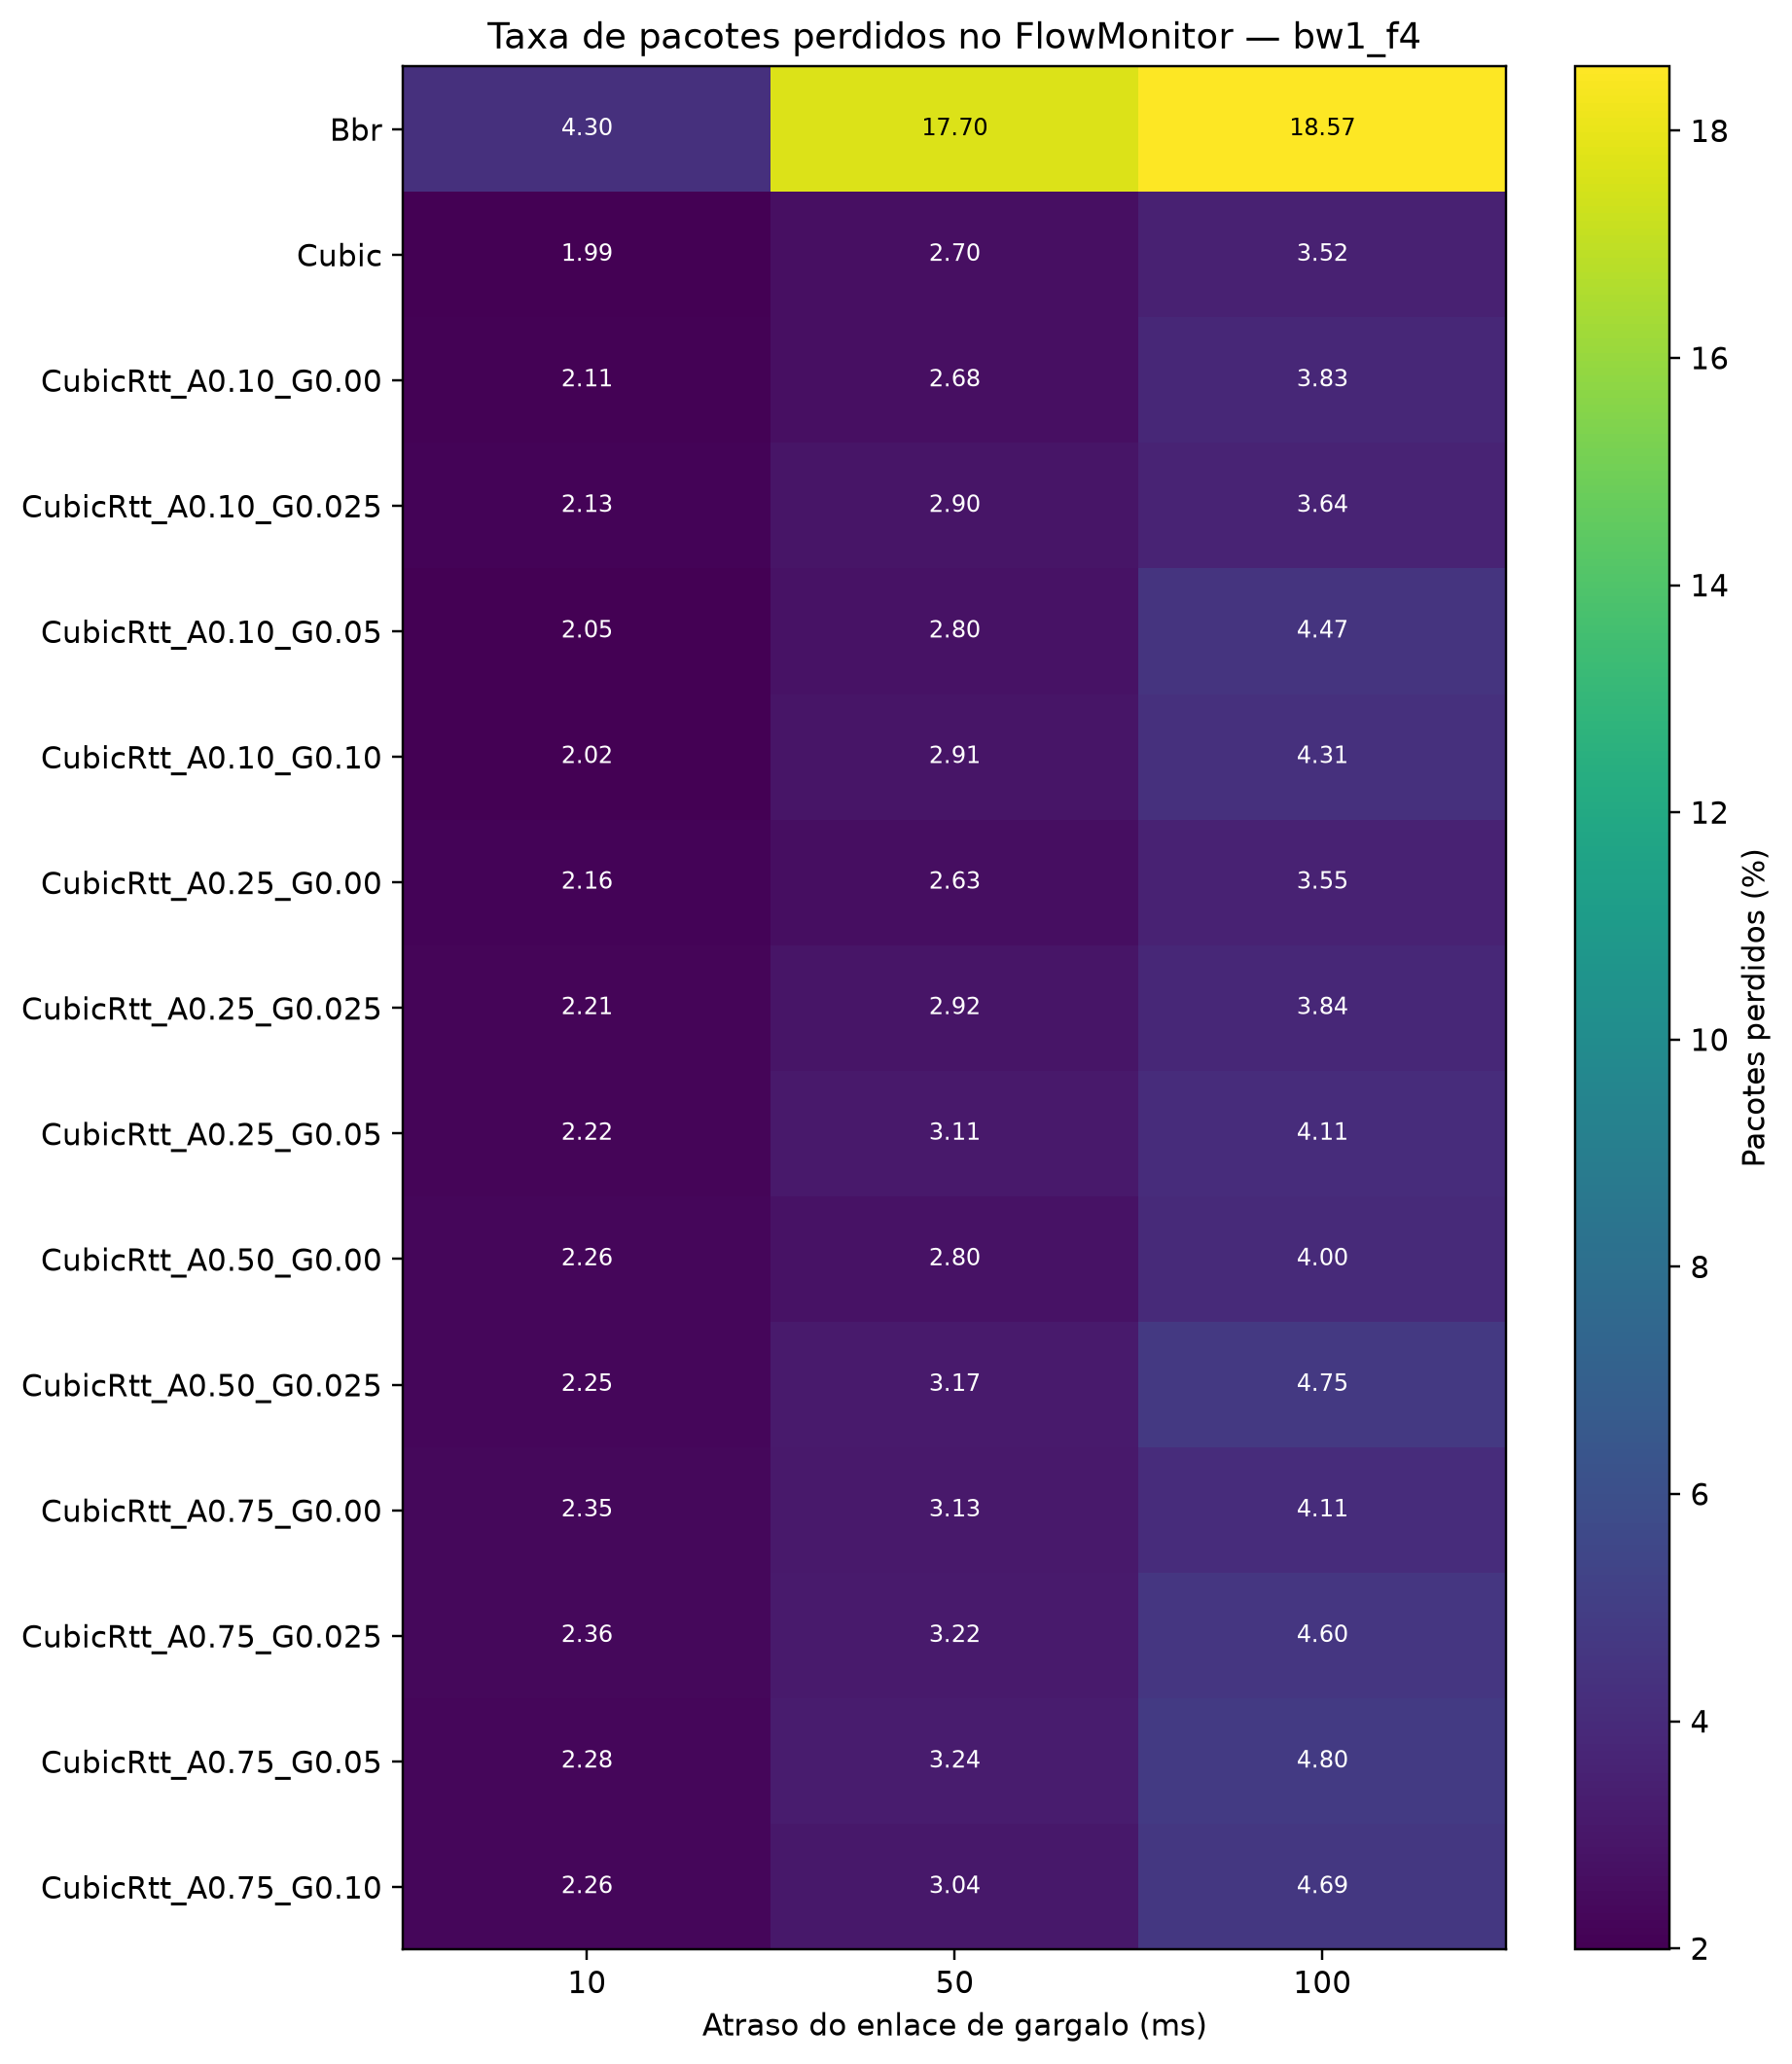
\includegraphics[width=0.88\textwidth]{bw1_f4_loss_rate_pct.png}
\caption{Taxa de perda de pacotes no cenário \texttt{bw1\_f4}.}
\label{fig:bw1-loss}
\end{figure}

\begin{figure}[p]
\centering
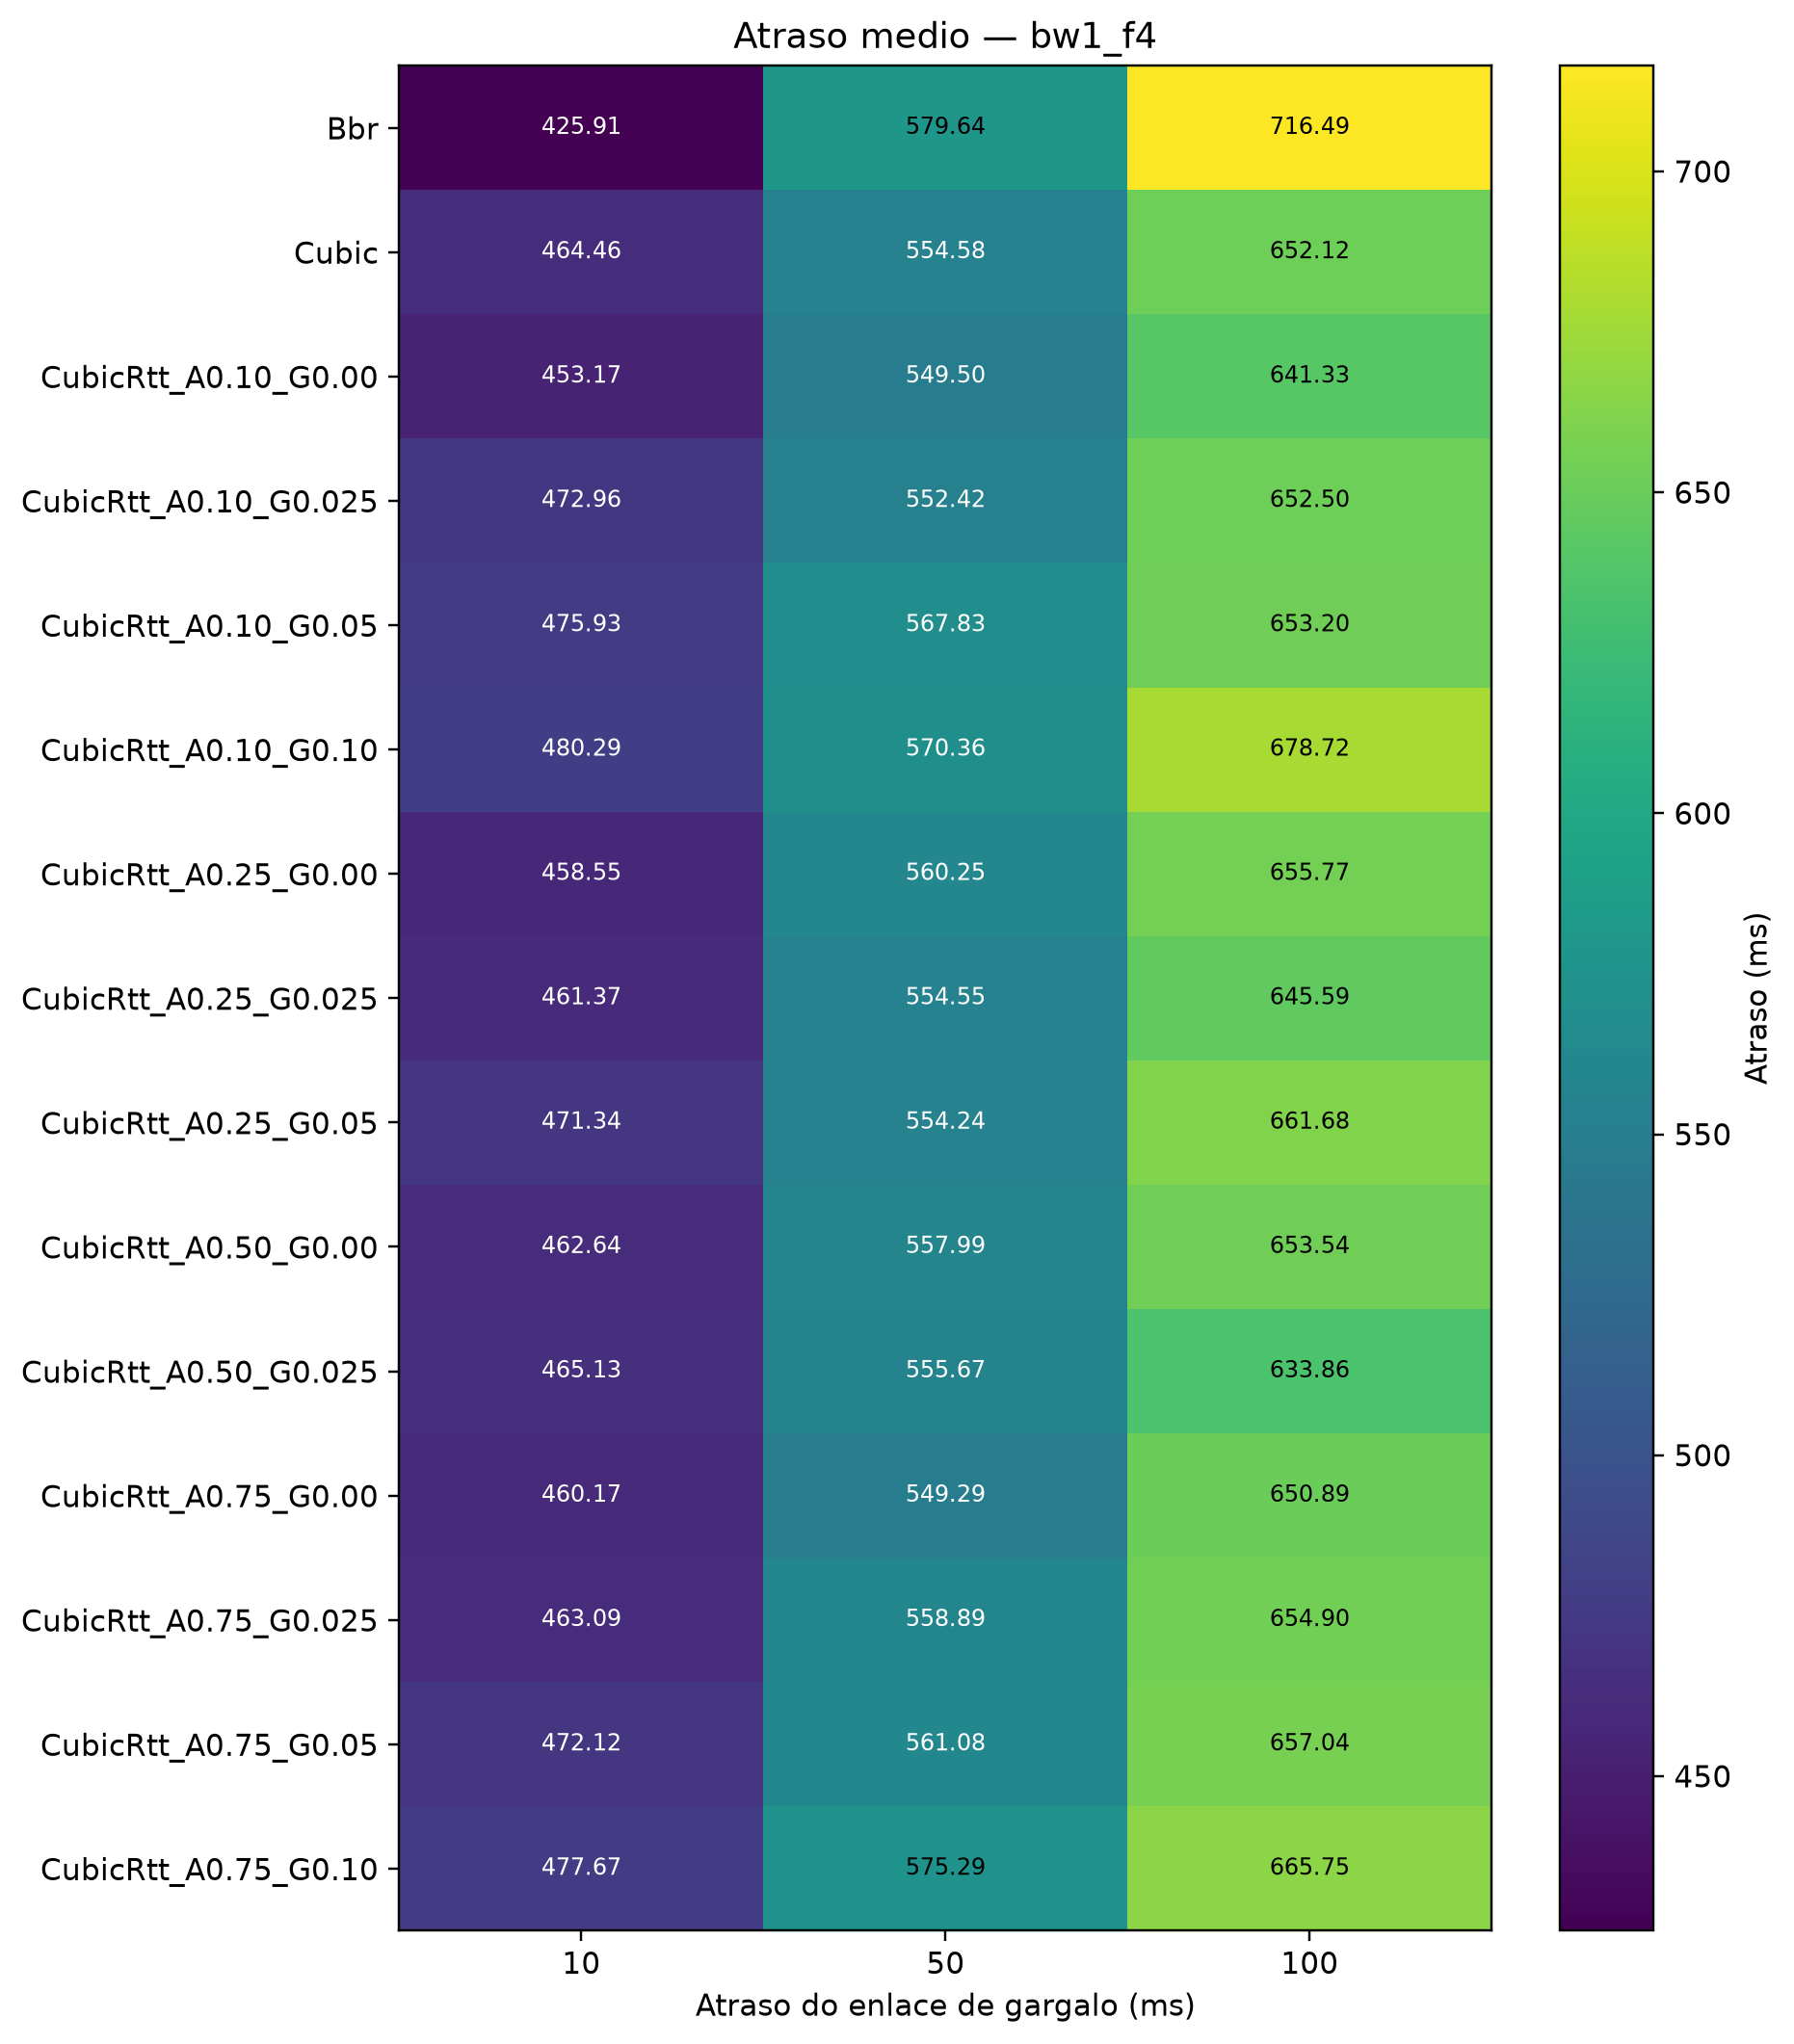
\includegraphics[width=0.88\textwidth]{bw1_f4_avg_delay_ms.png}
\caption{Atraso médio no cenário \texttt{bw1\_f4}.}
\label{fig:bw1-delay}
\end{figure}

\begin{figure}[p]
\centering
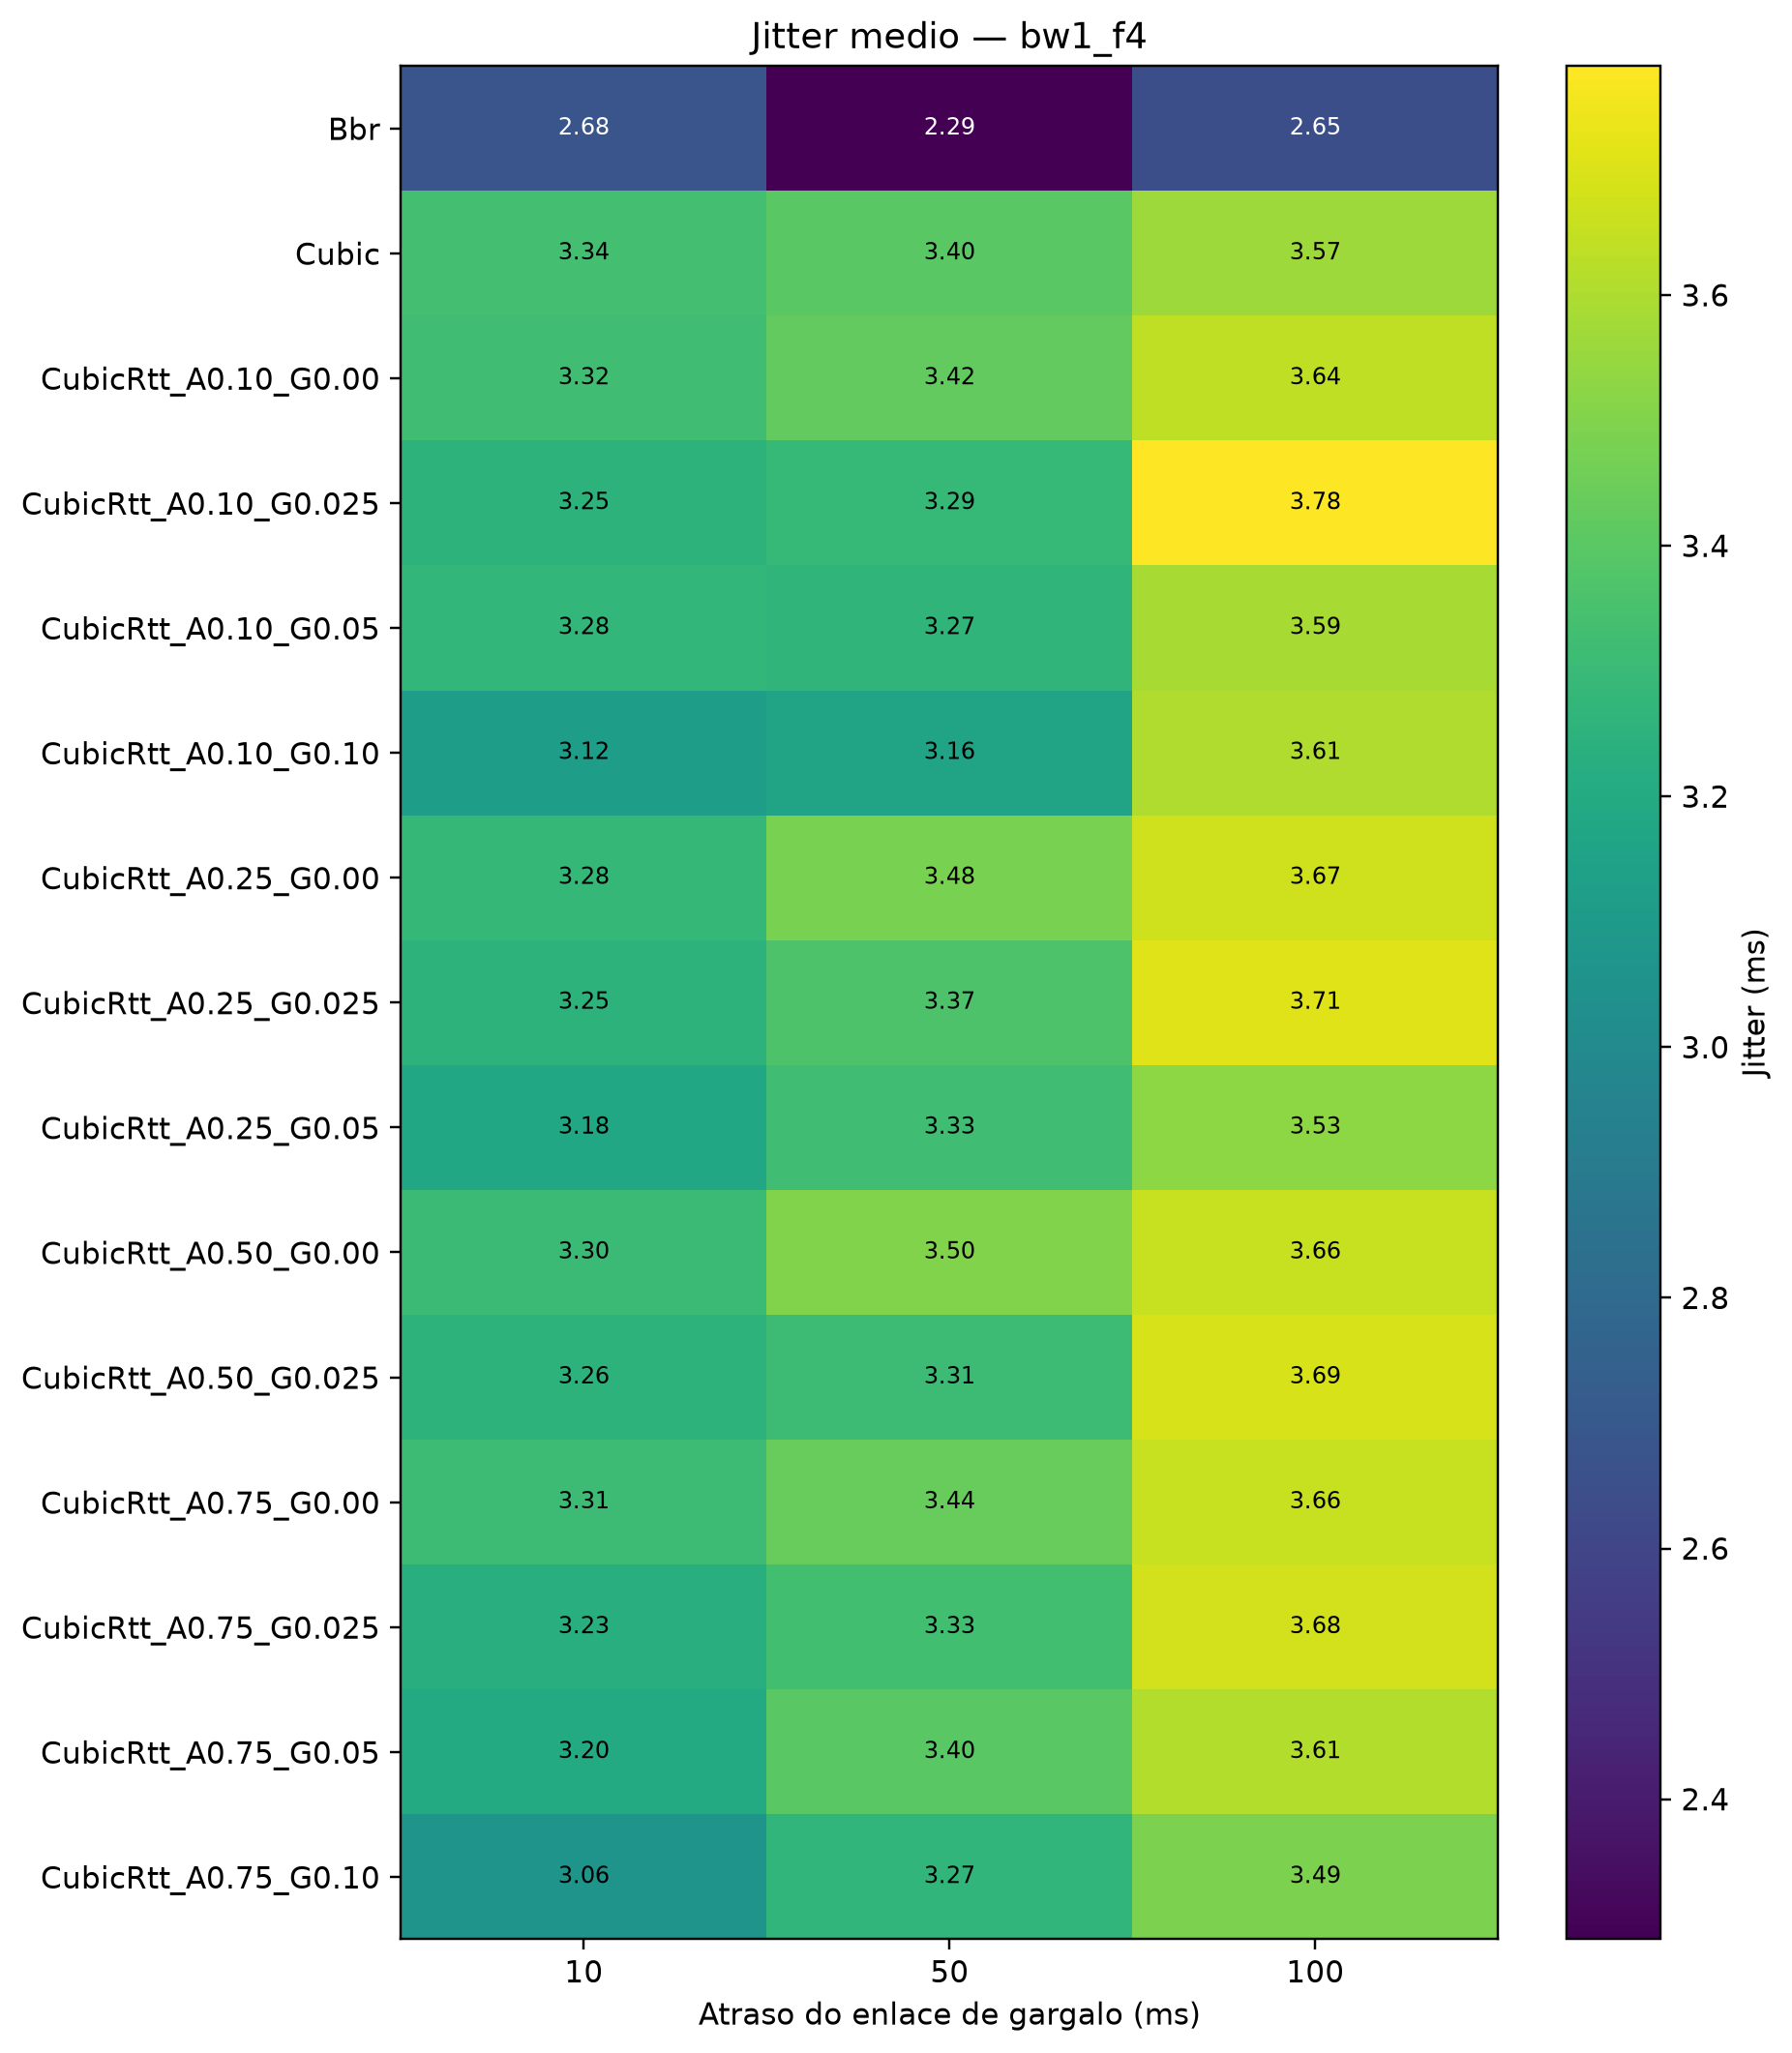
\includegraphics[width=0.88\textwidth]{bw1_f4_avg_jitter_ms.png}
\caption{Jitter médio no cenário \texttt{bw1\_f4}.}
\label{fig:bw1-jitter}
\end{figure}

\begin{figure}[p]
\centering
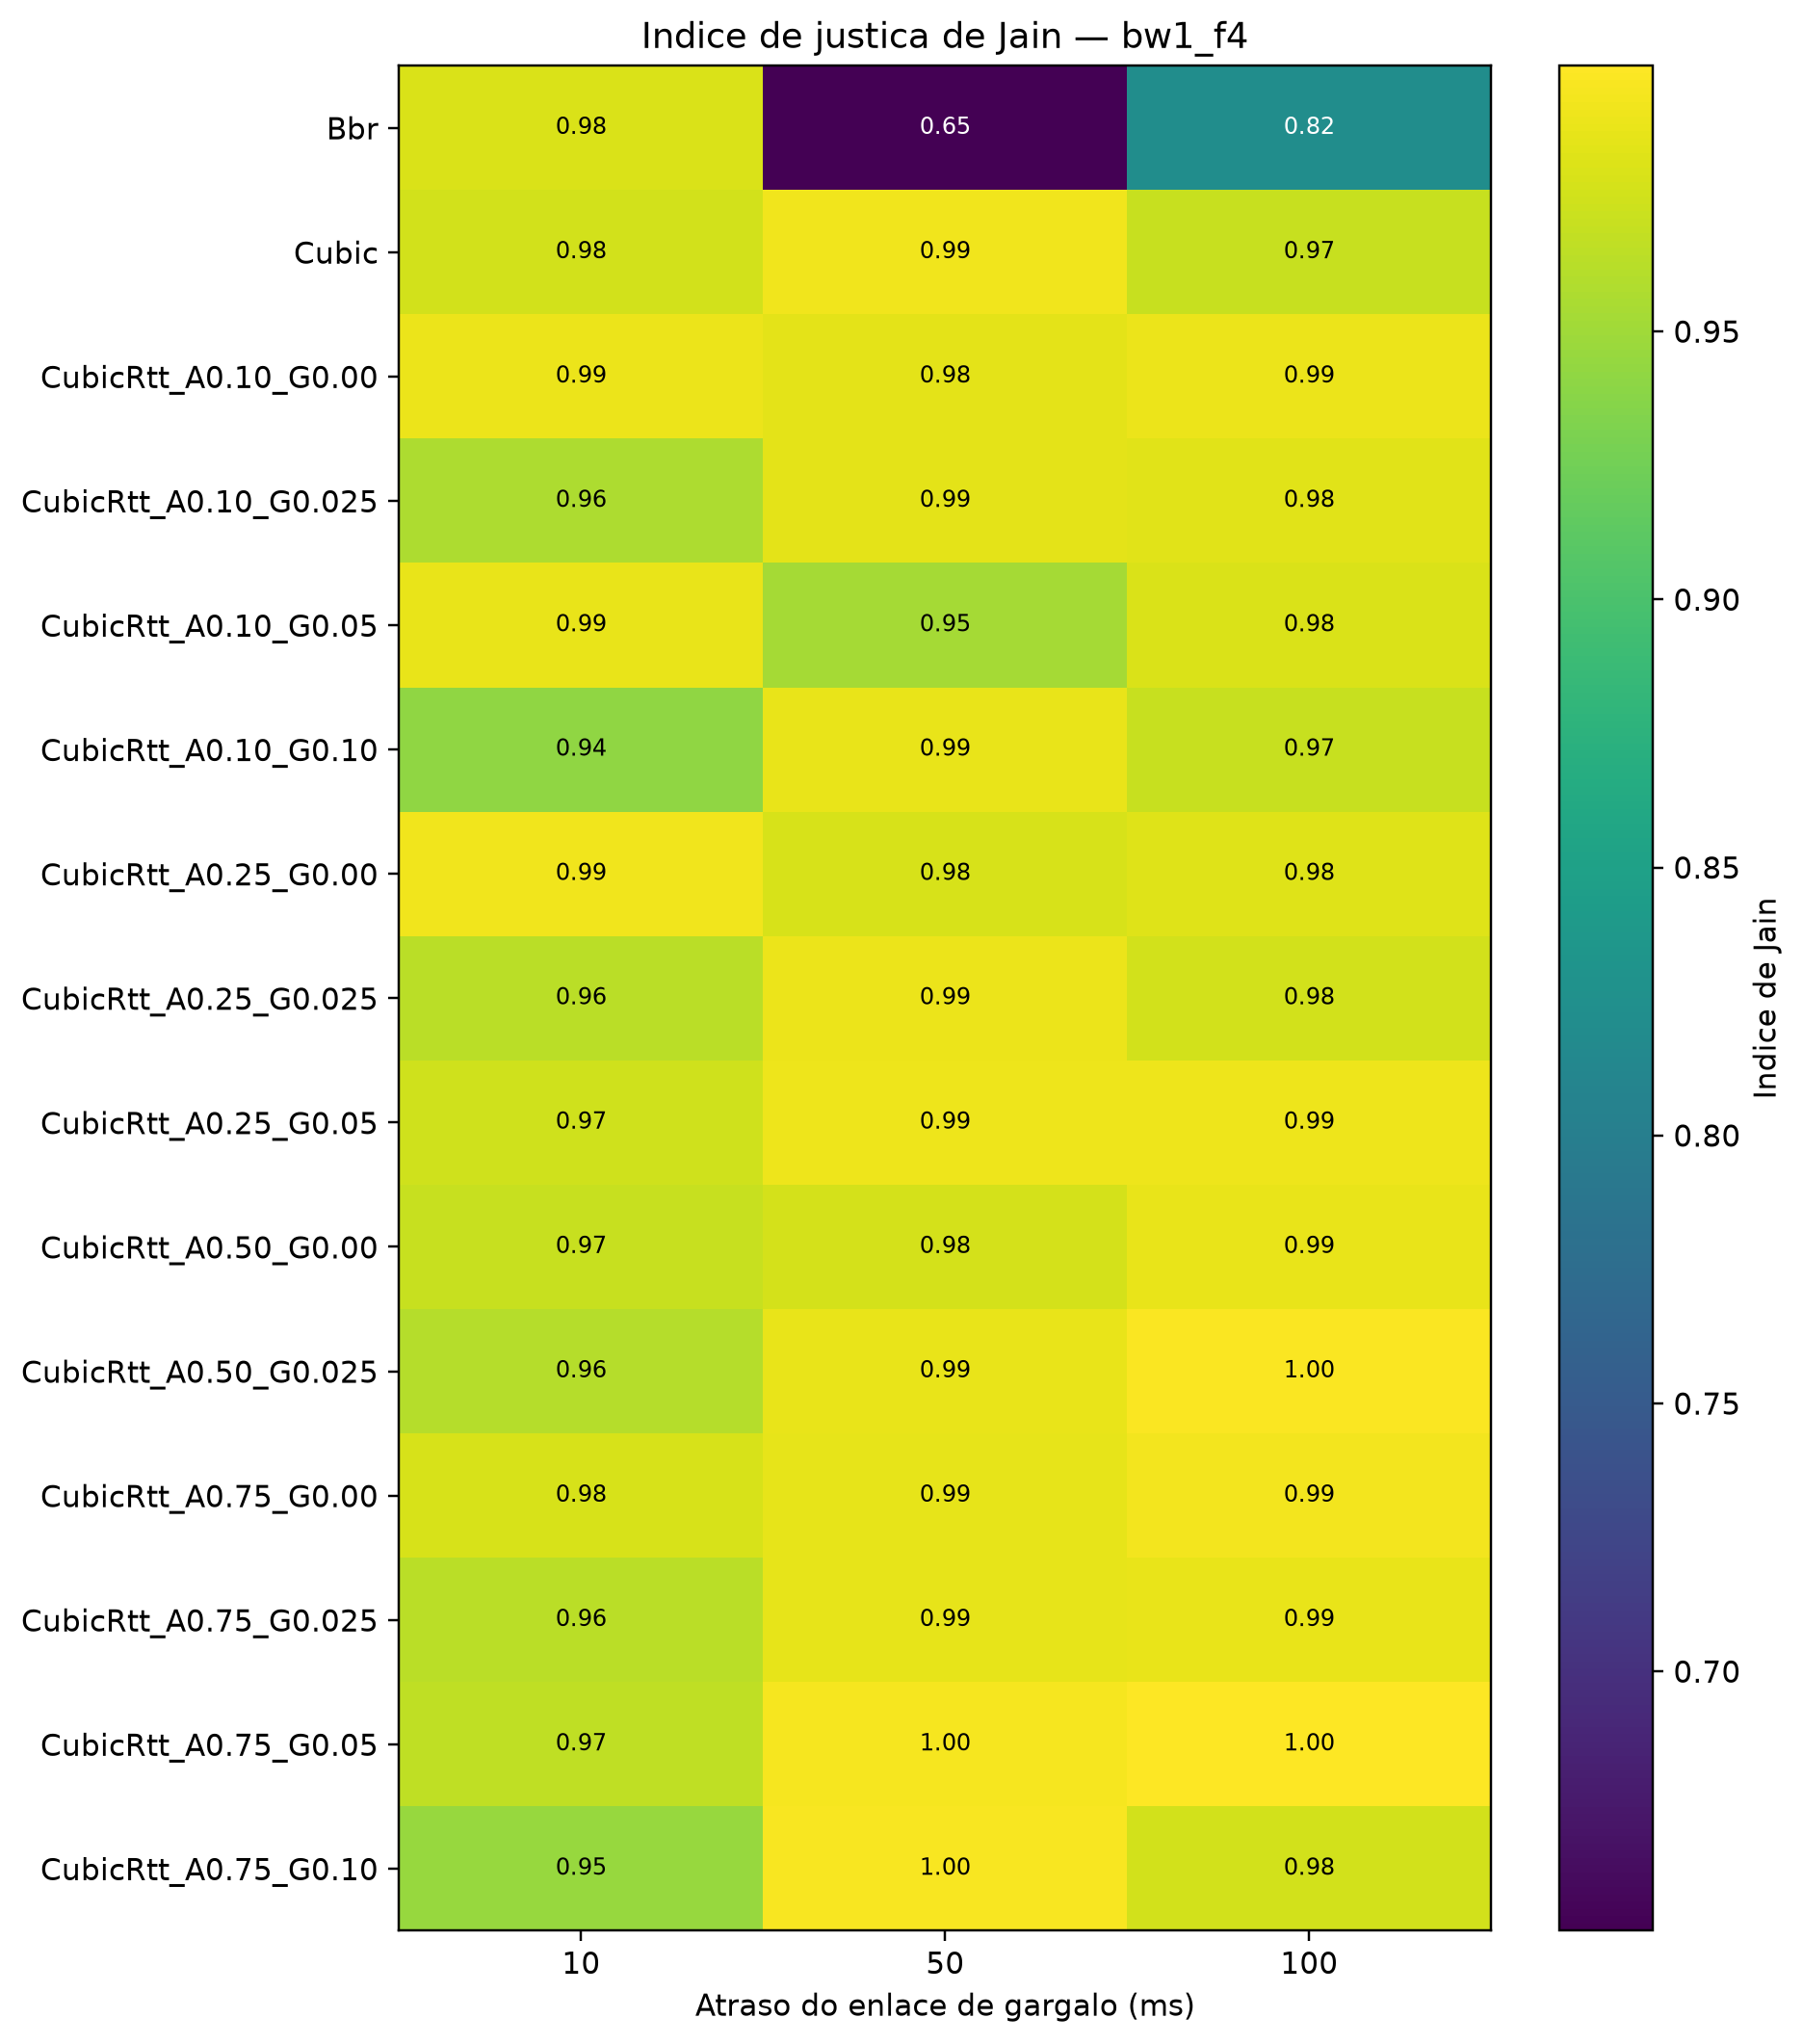
\includegraphics[width=0.88\textwidth]{bw1_f4_jain_fairness.png}
\caption{Índice de Justiça de Jain no cenário \texttt{bw1\_f4}.}
\label{fig:bw1-jain}
\end{figure}

\section{Cenário bw2\_f8}

\begin{figure}[p]
\centering
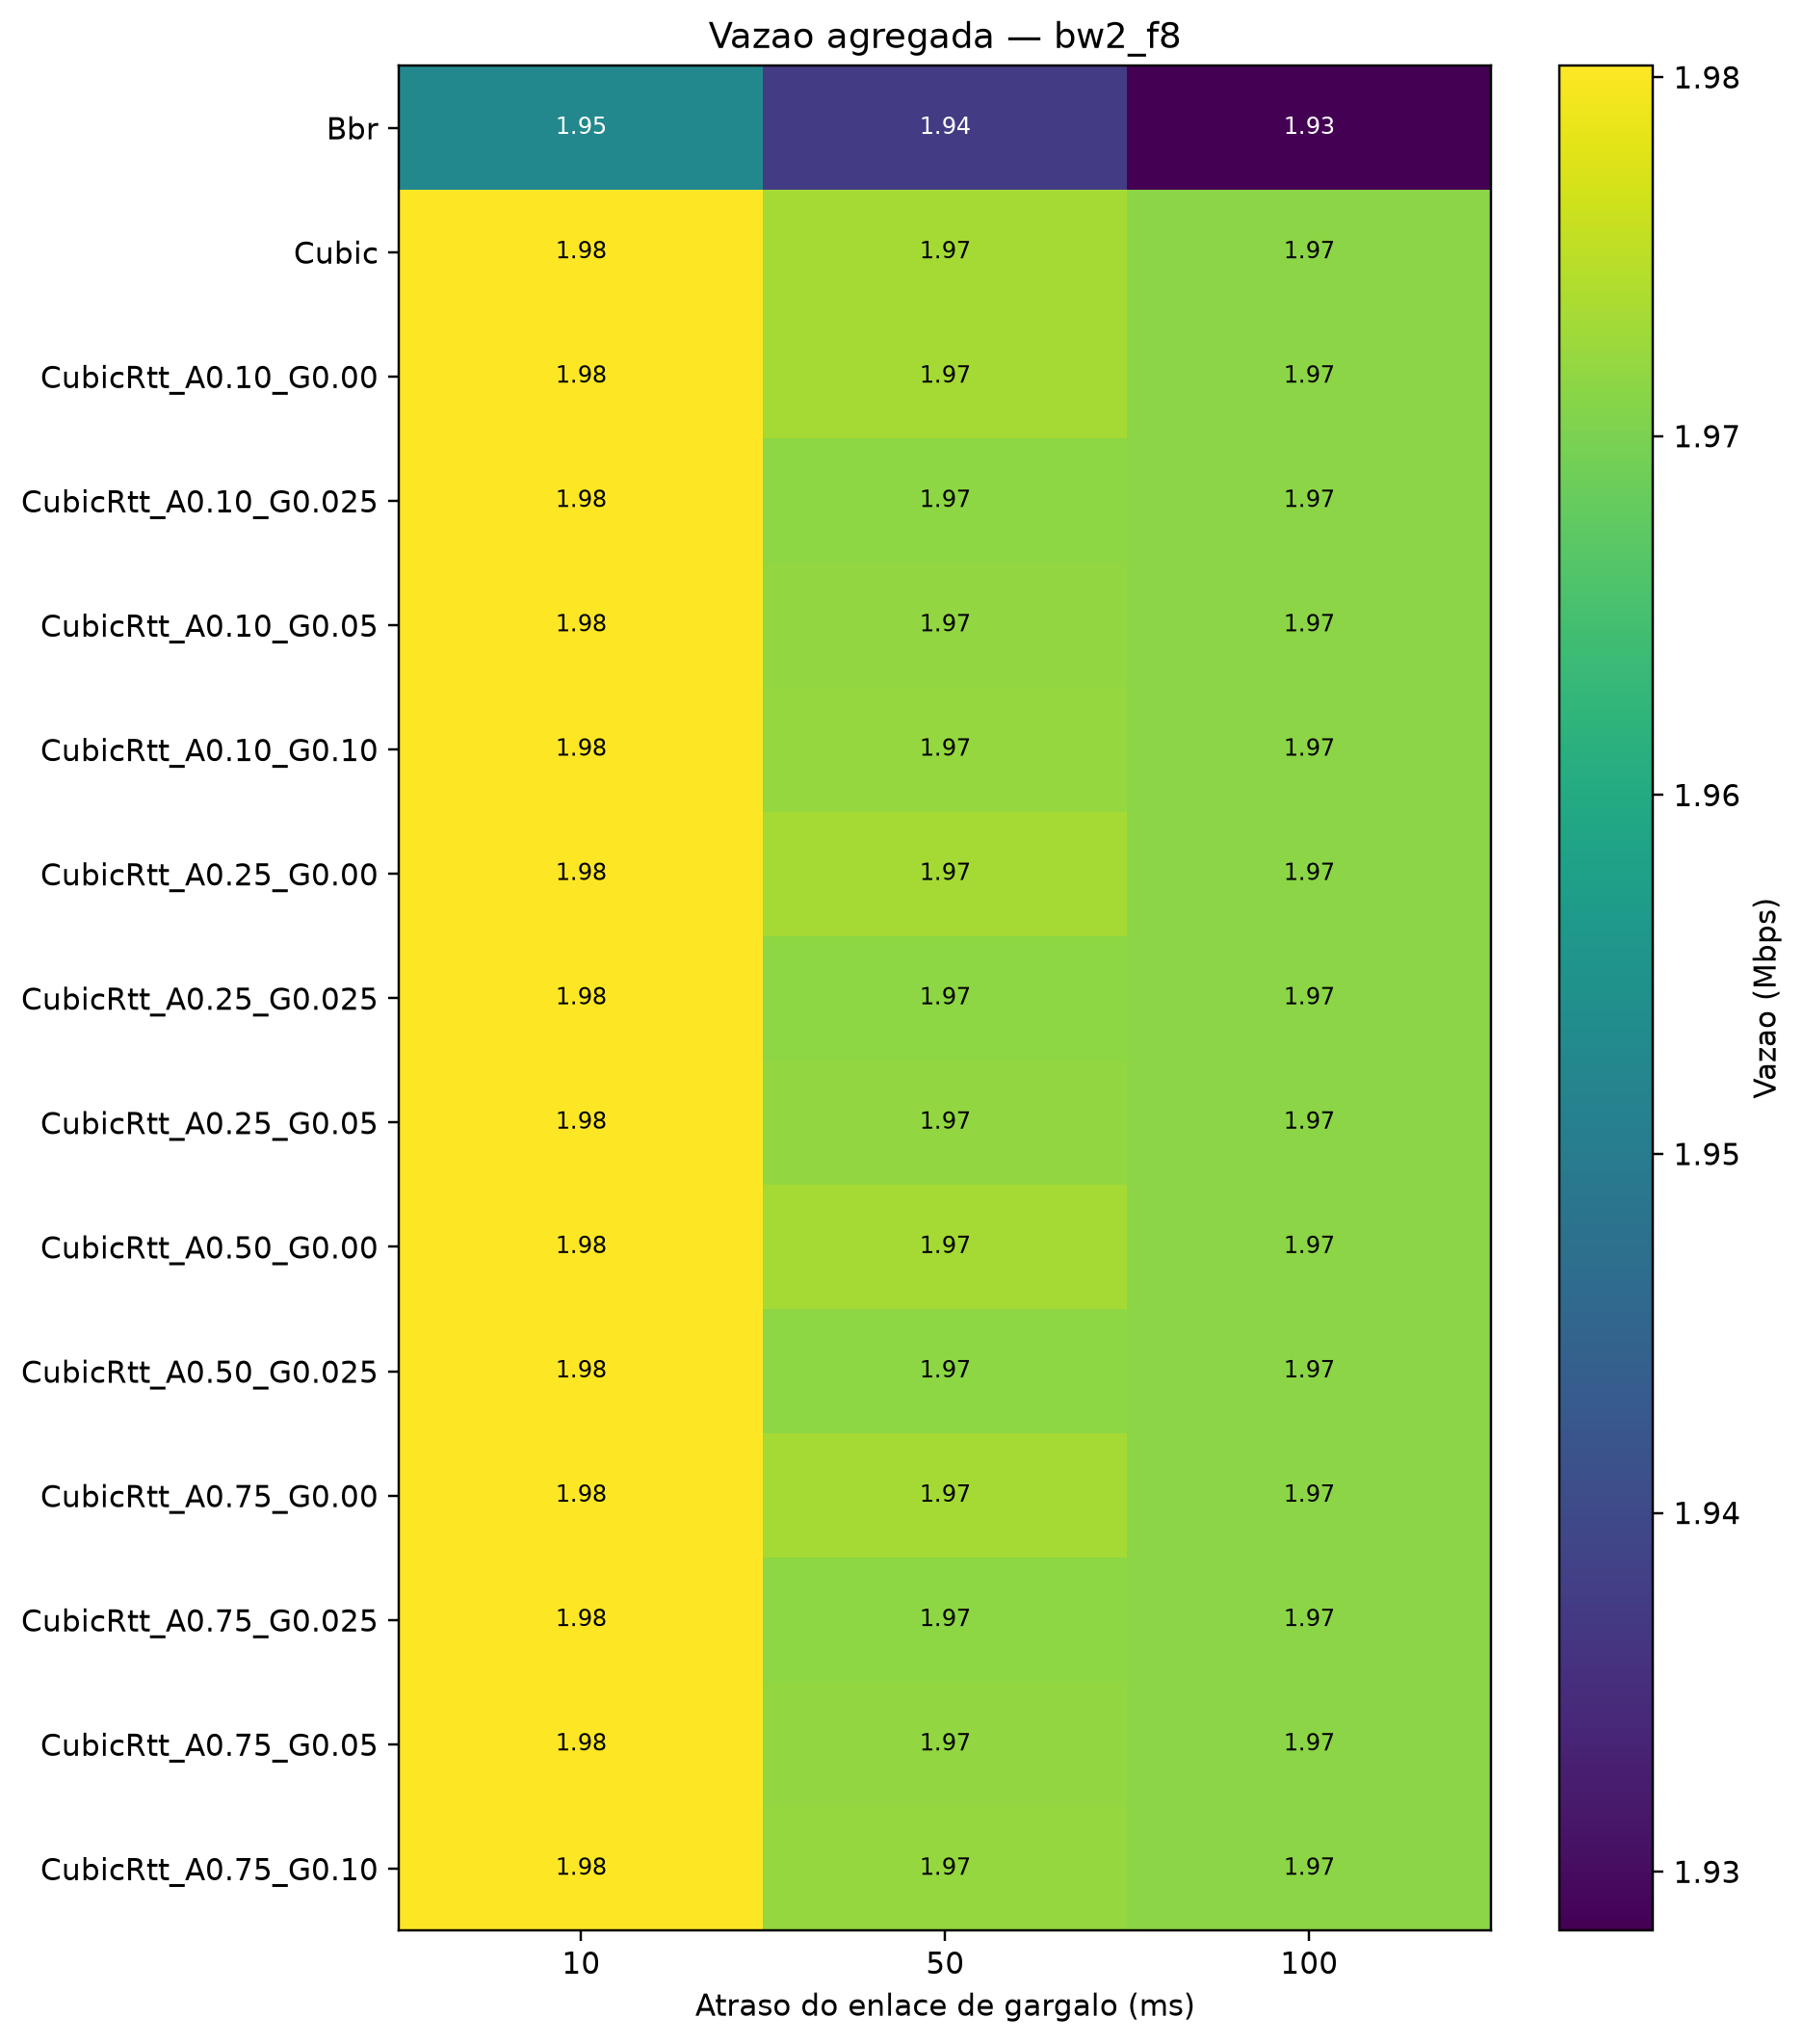
\includegraphics[width=0.88\textwidth]{bw2_f8_throughput_mbps.png}
\caption{Vazão agregada no cenário \texttt{bw2\_f8}.}
\label{fig:bw2-throughput}
\end{figure}

\begin{figure}[p]
\centering
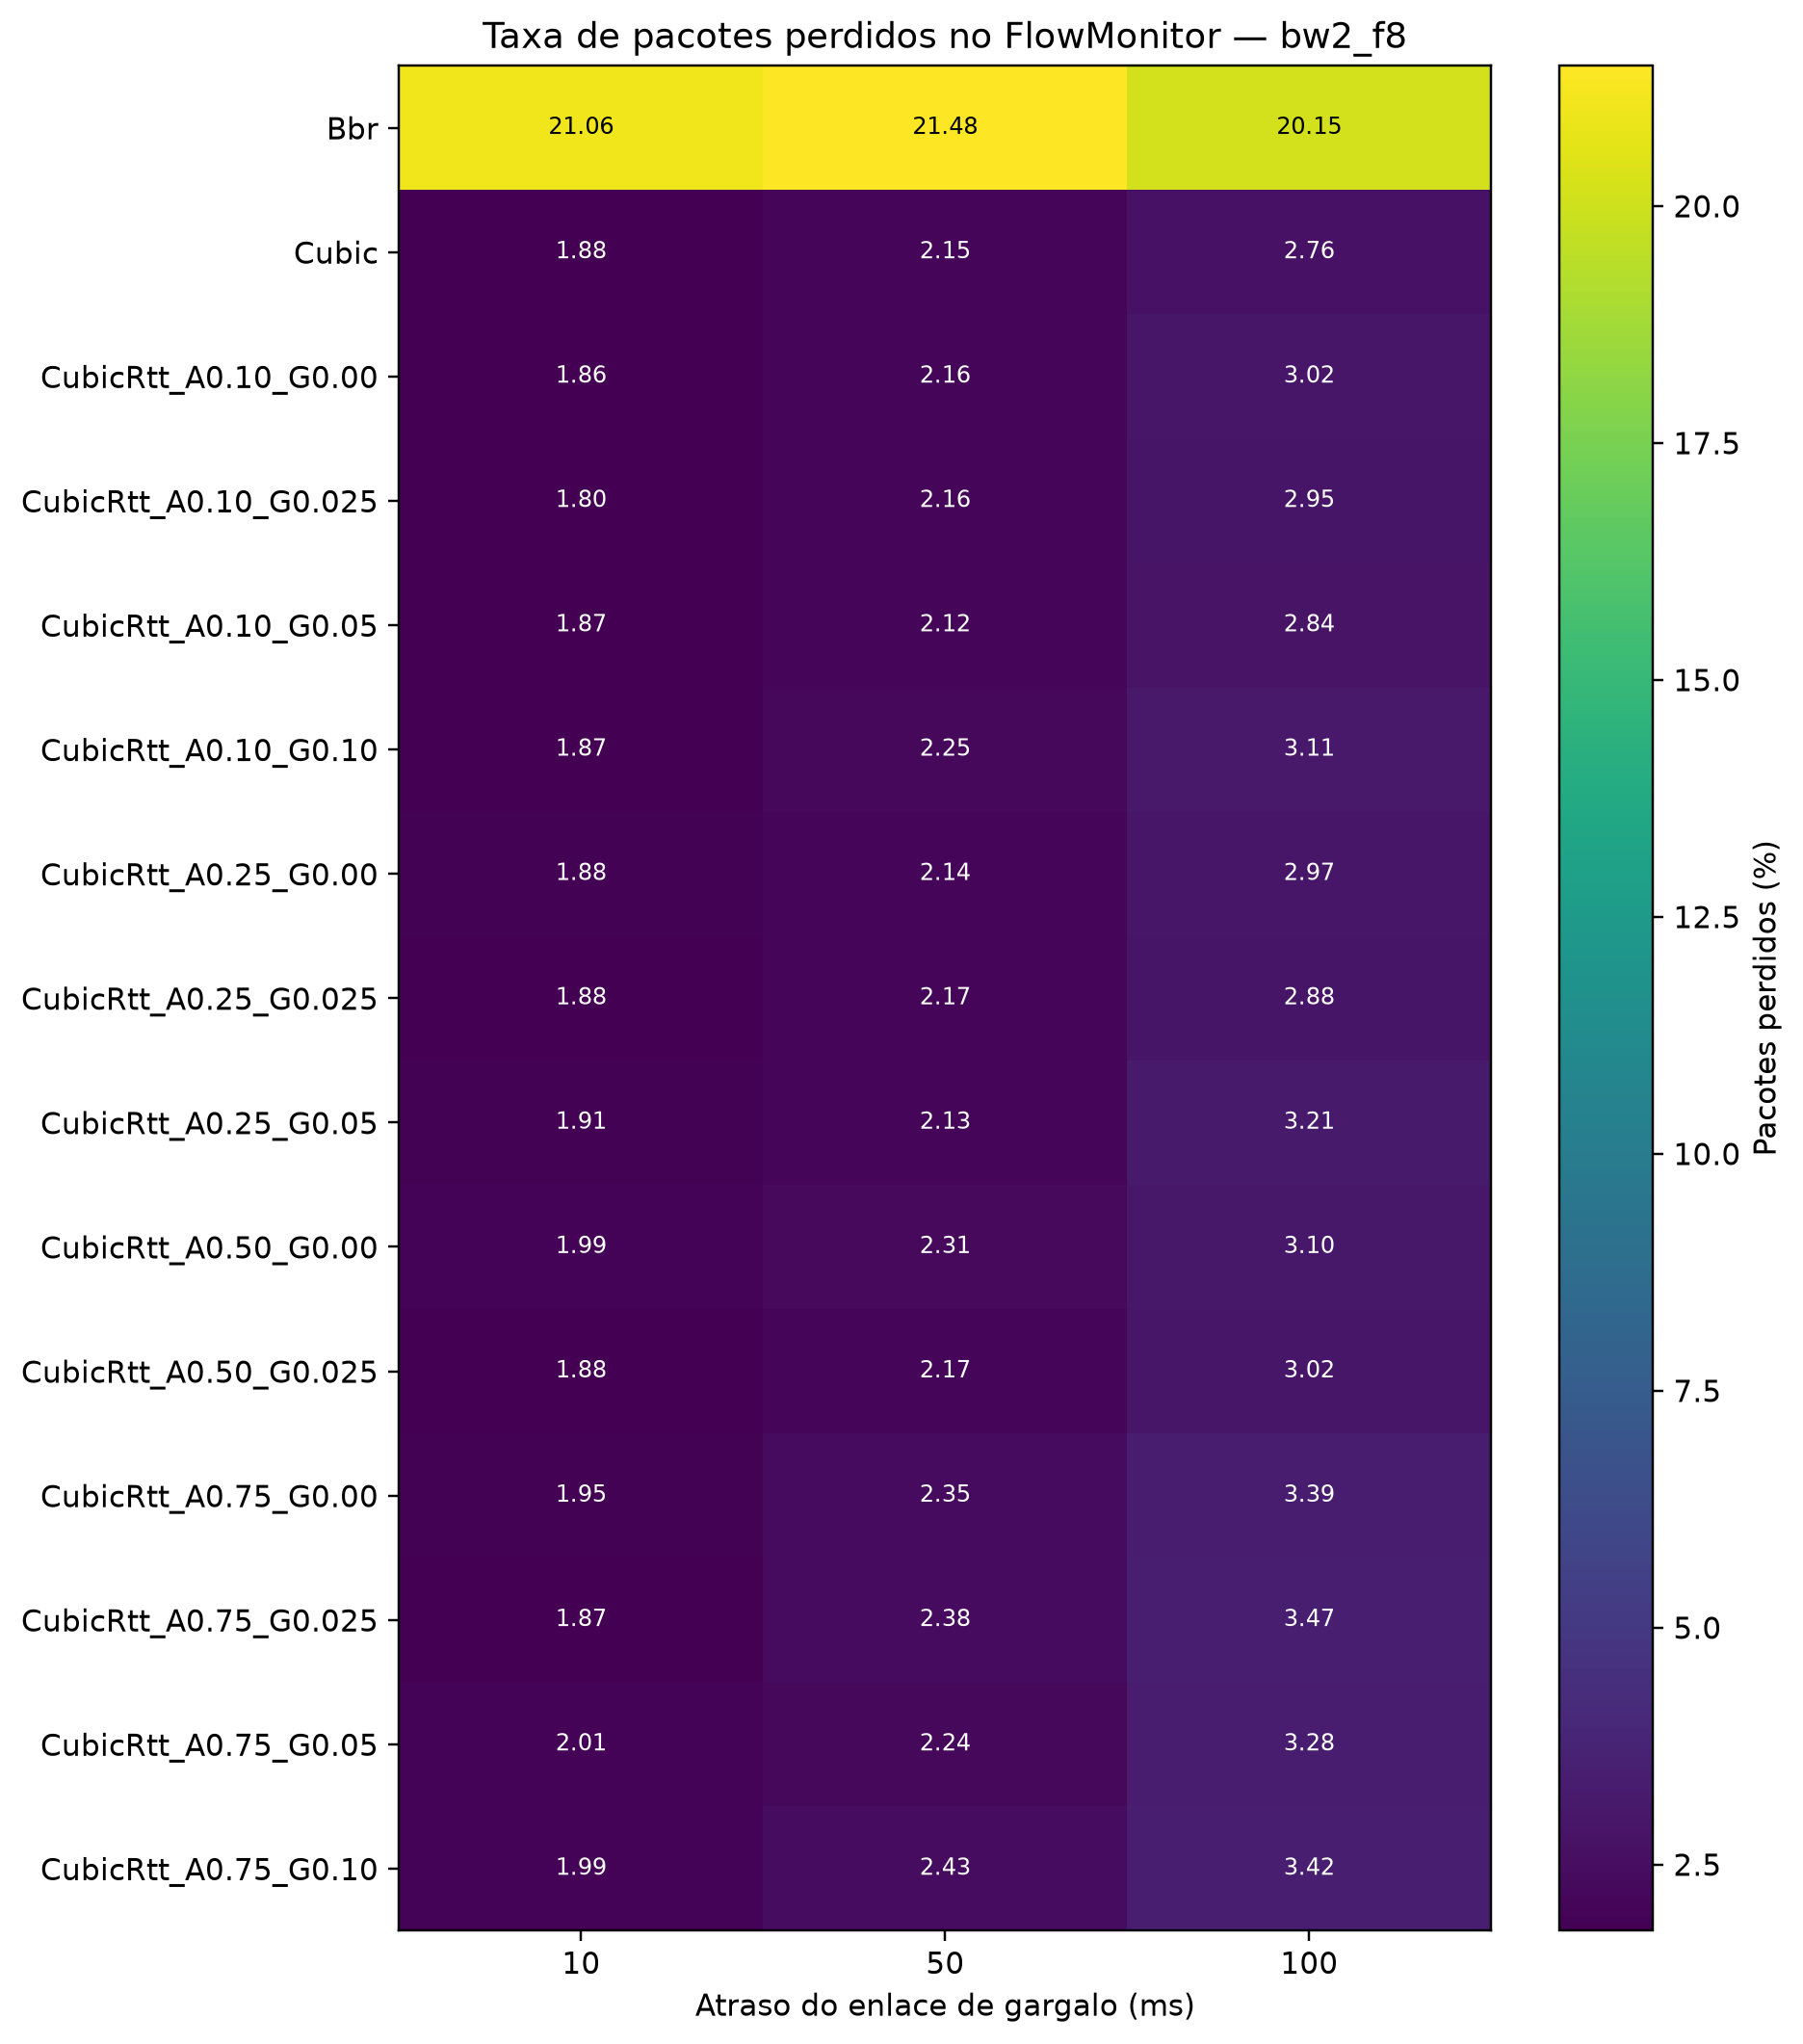
\includegraphics[width=0.88\textwidth]{bw2_f8_loss_rate_pct.png}
\caption{Taxa de perda de pacotes no cenário \texttt{bw2\_f8}.}
\label{fig:bw2-loss}
\end{figure}

\begin{figure}[p]
\centering
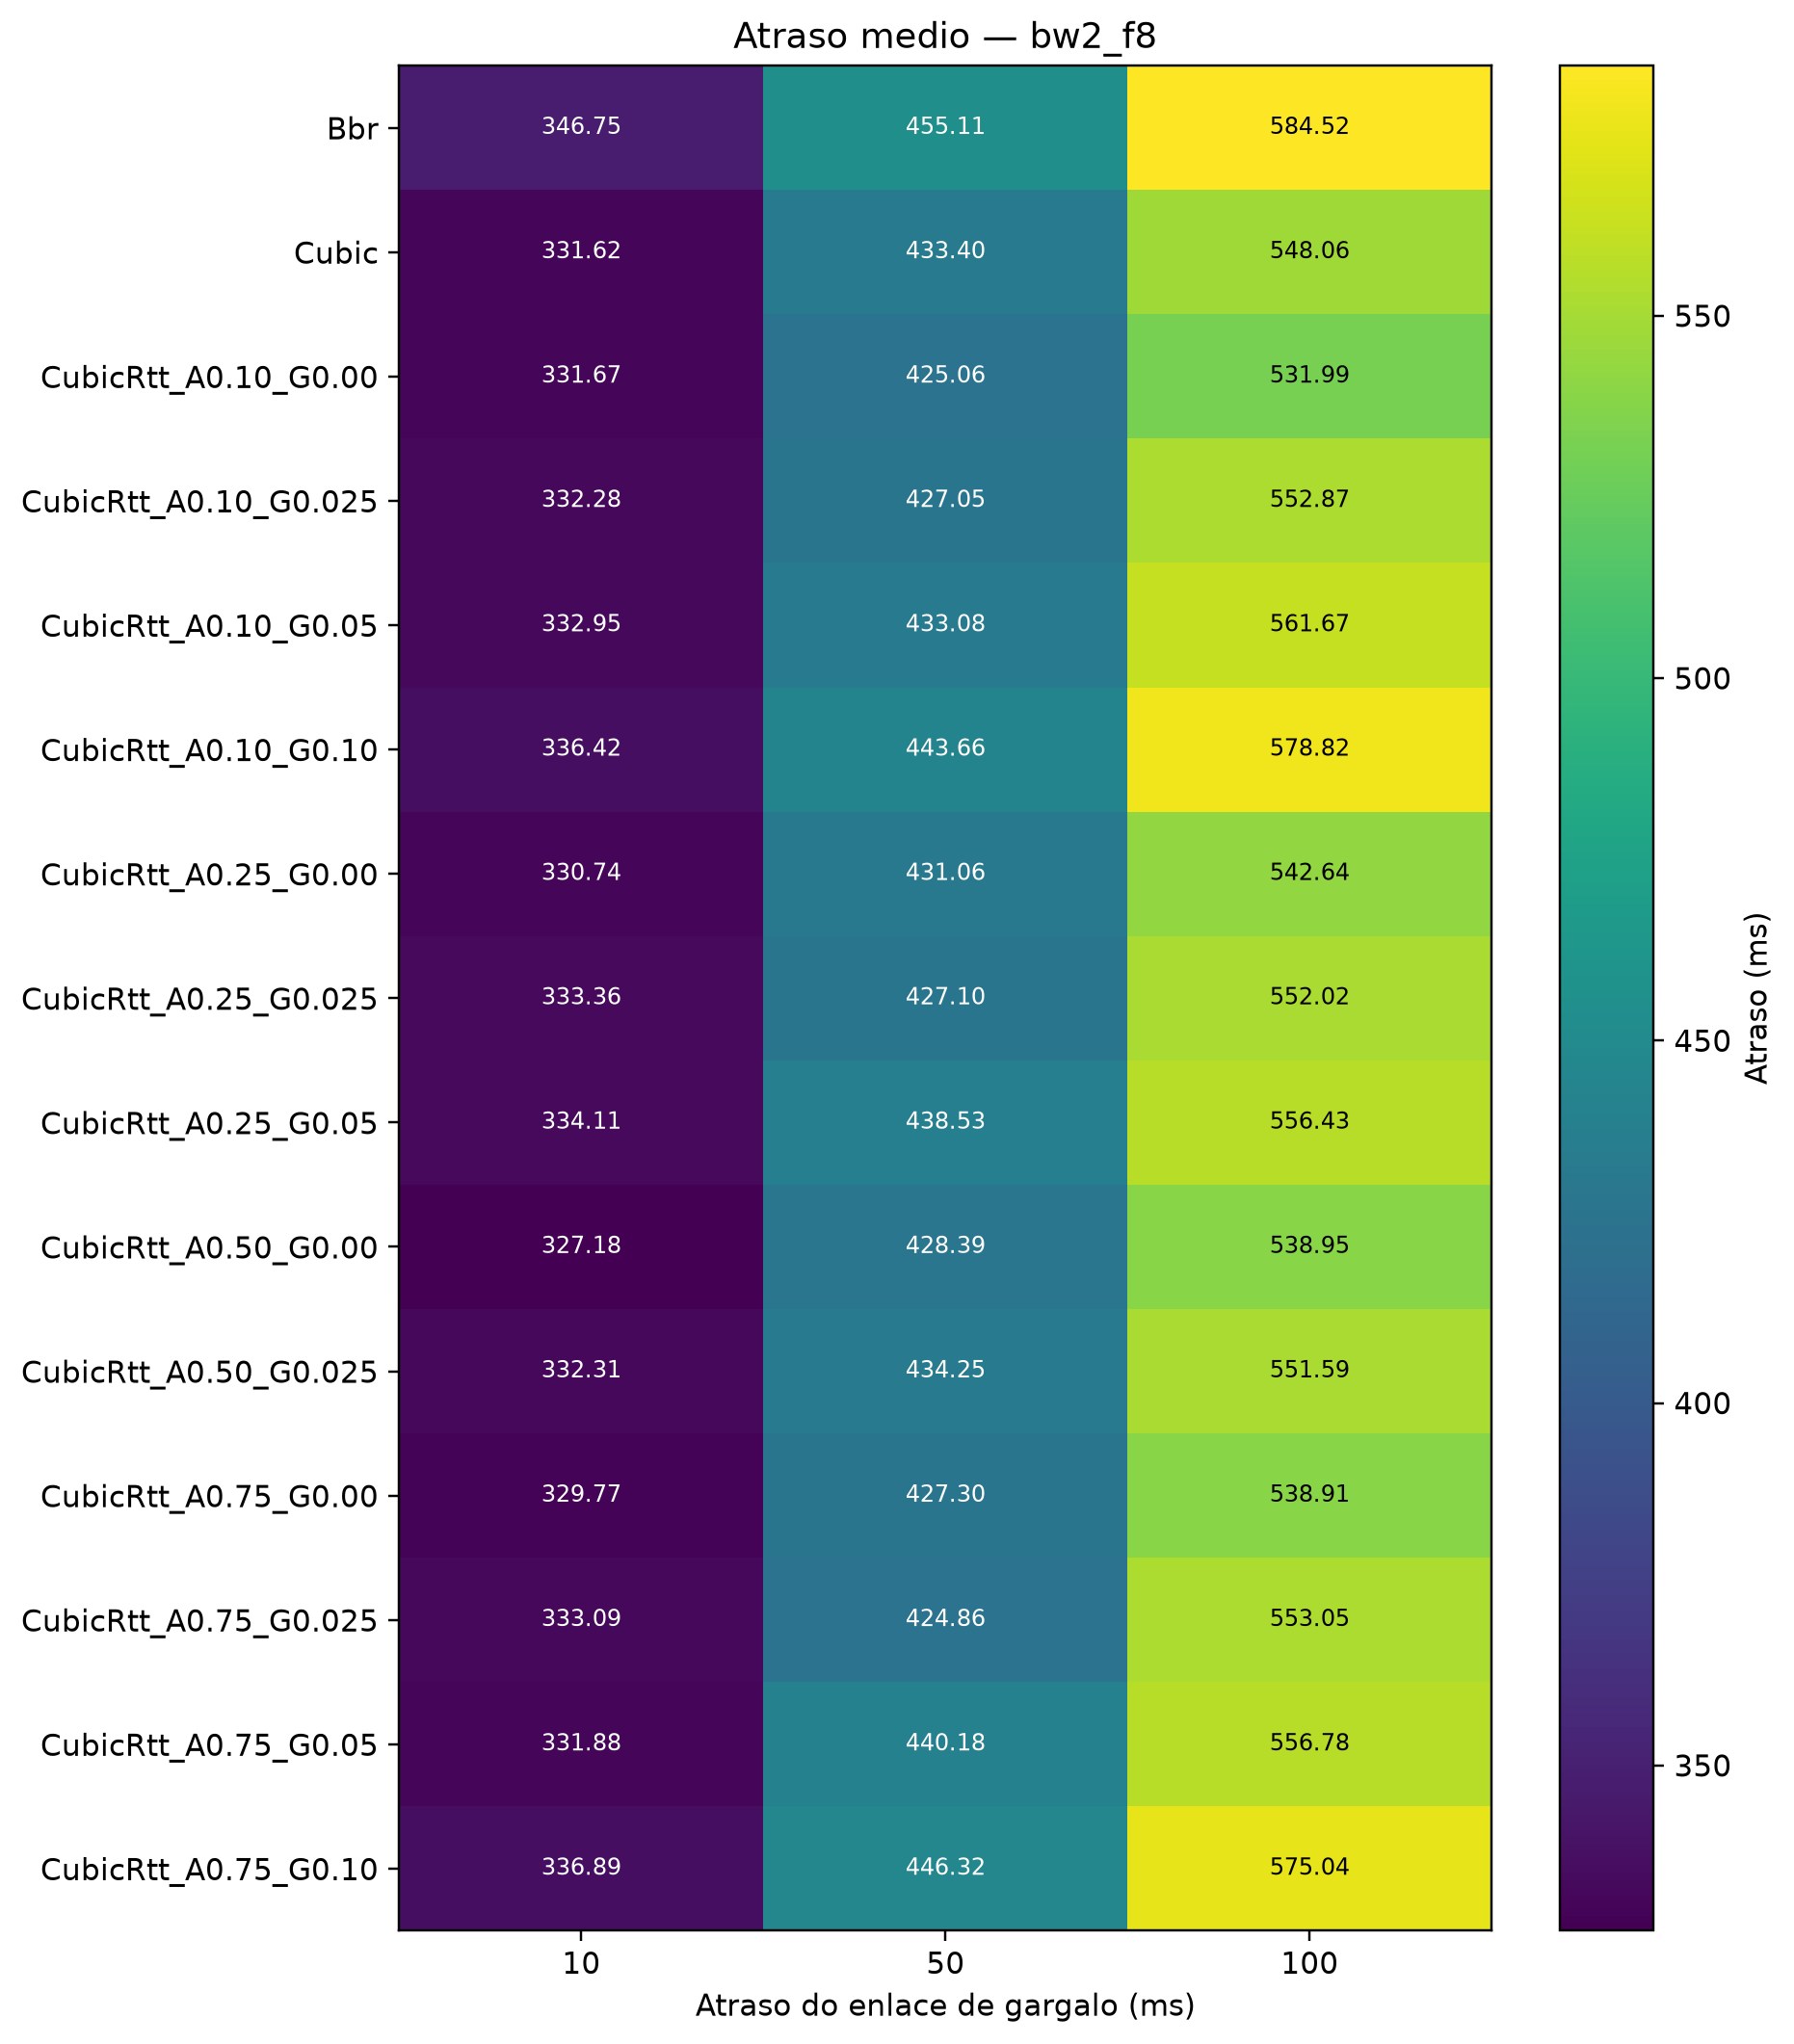
\includegraphics[width=0.88\textwidth]{bw2_f8_avg_delay_ms.png}
\caption{Atraso médio no cenário \texttt{bw2\_f8}.}
\label{fig:bw2-delay}
\end{figure}

\begin{figure}[p]
\centering
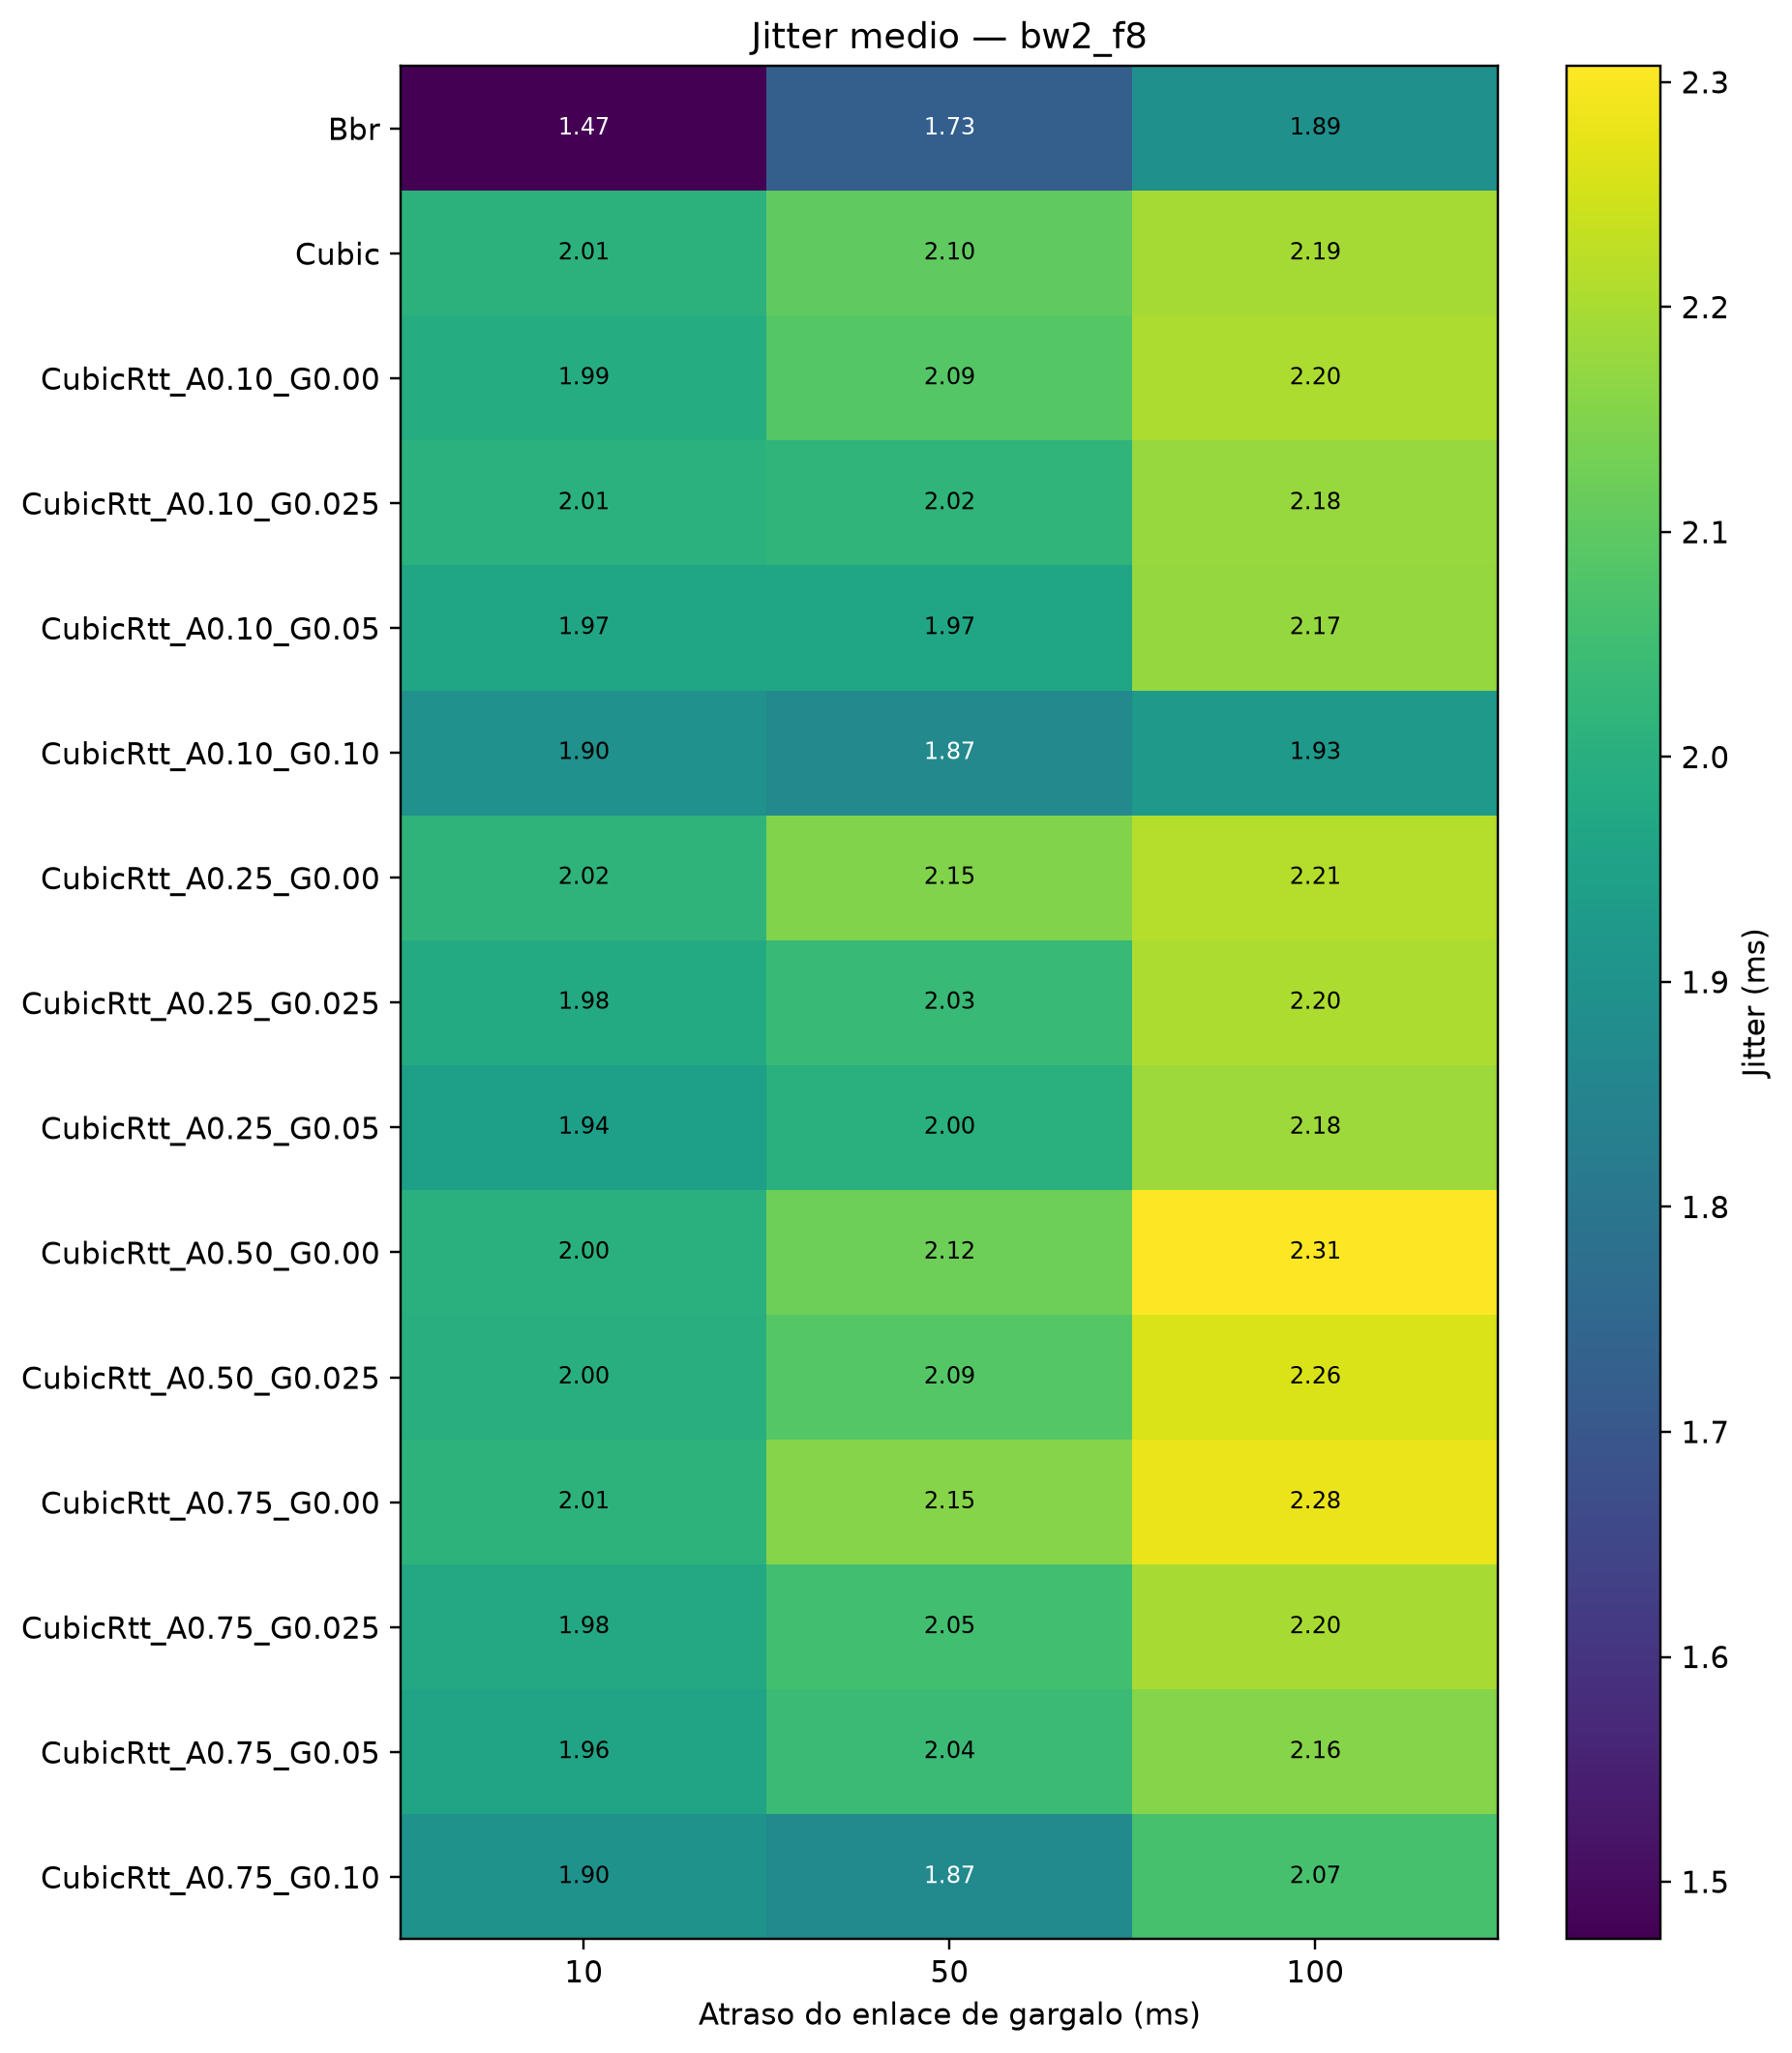
\includegraphics[width=0.88\textwidth]{bw2_f8_avg_jitter_ms.png}
\caption{Jitter médio no cenário \texttt{bw2\_f8}.}
\label{fig:bw2-jitter}
\end{figure}

\begin{figure}[p]
\centering
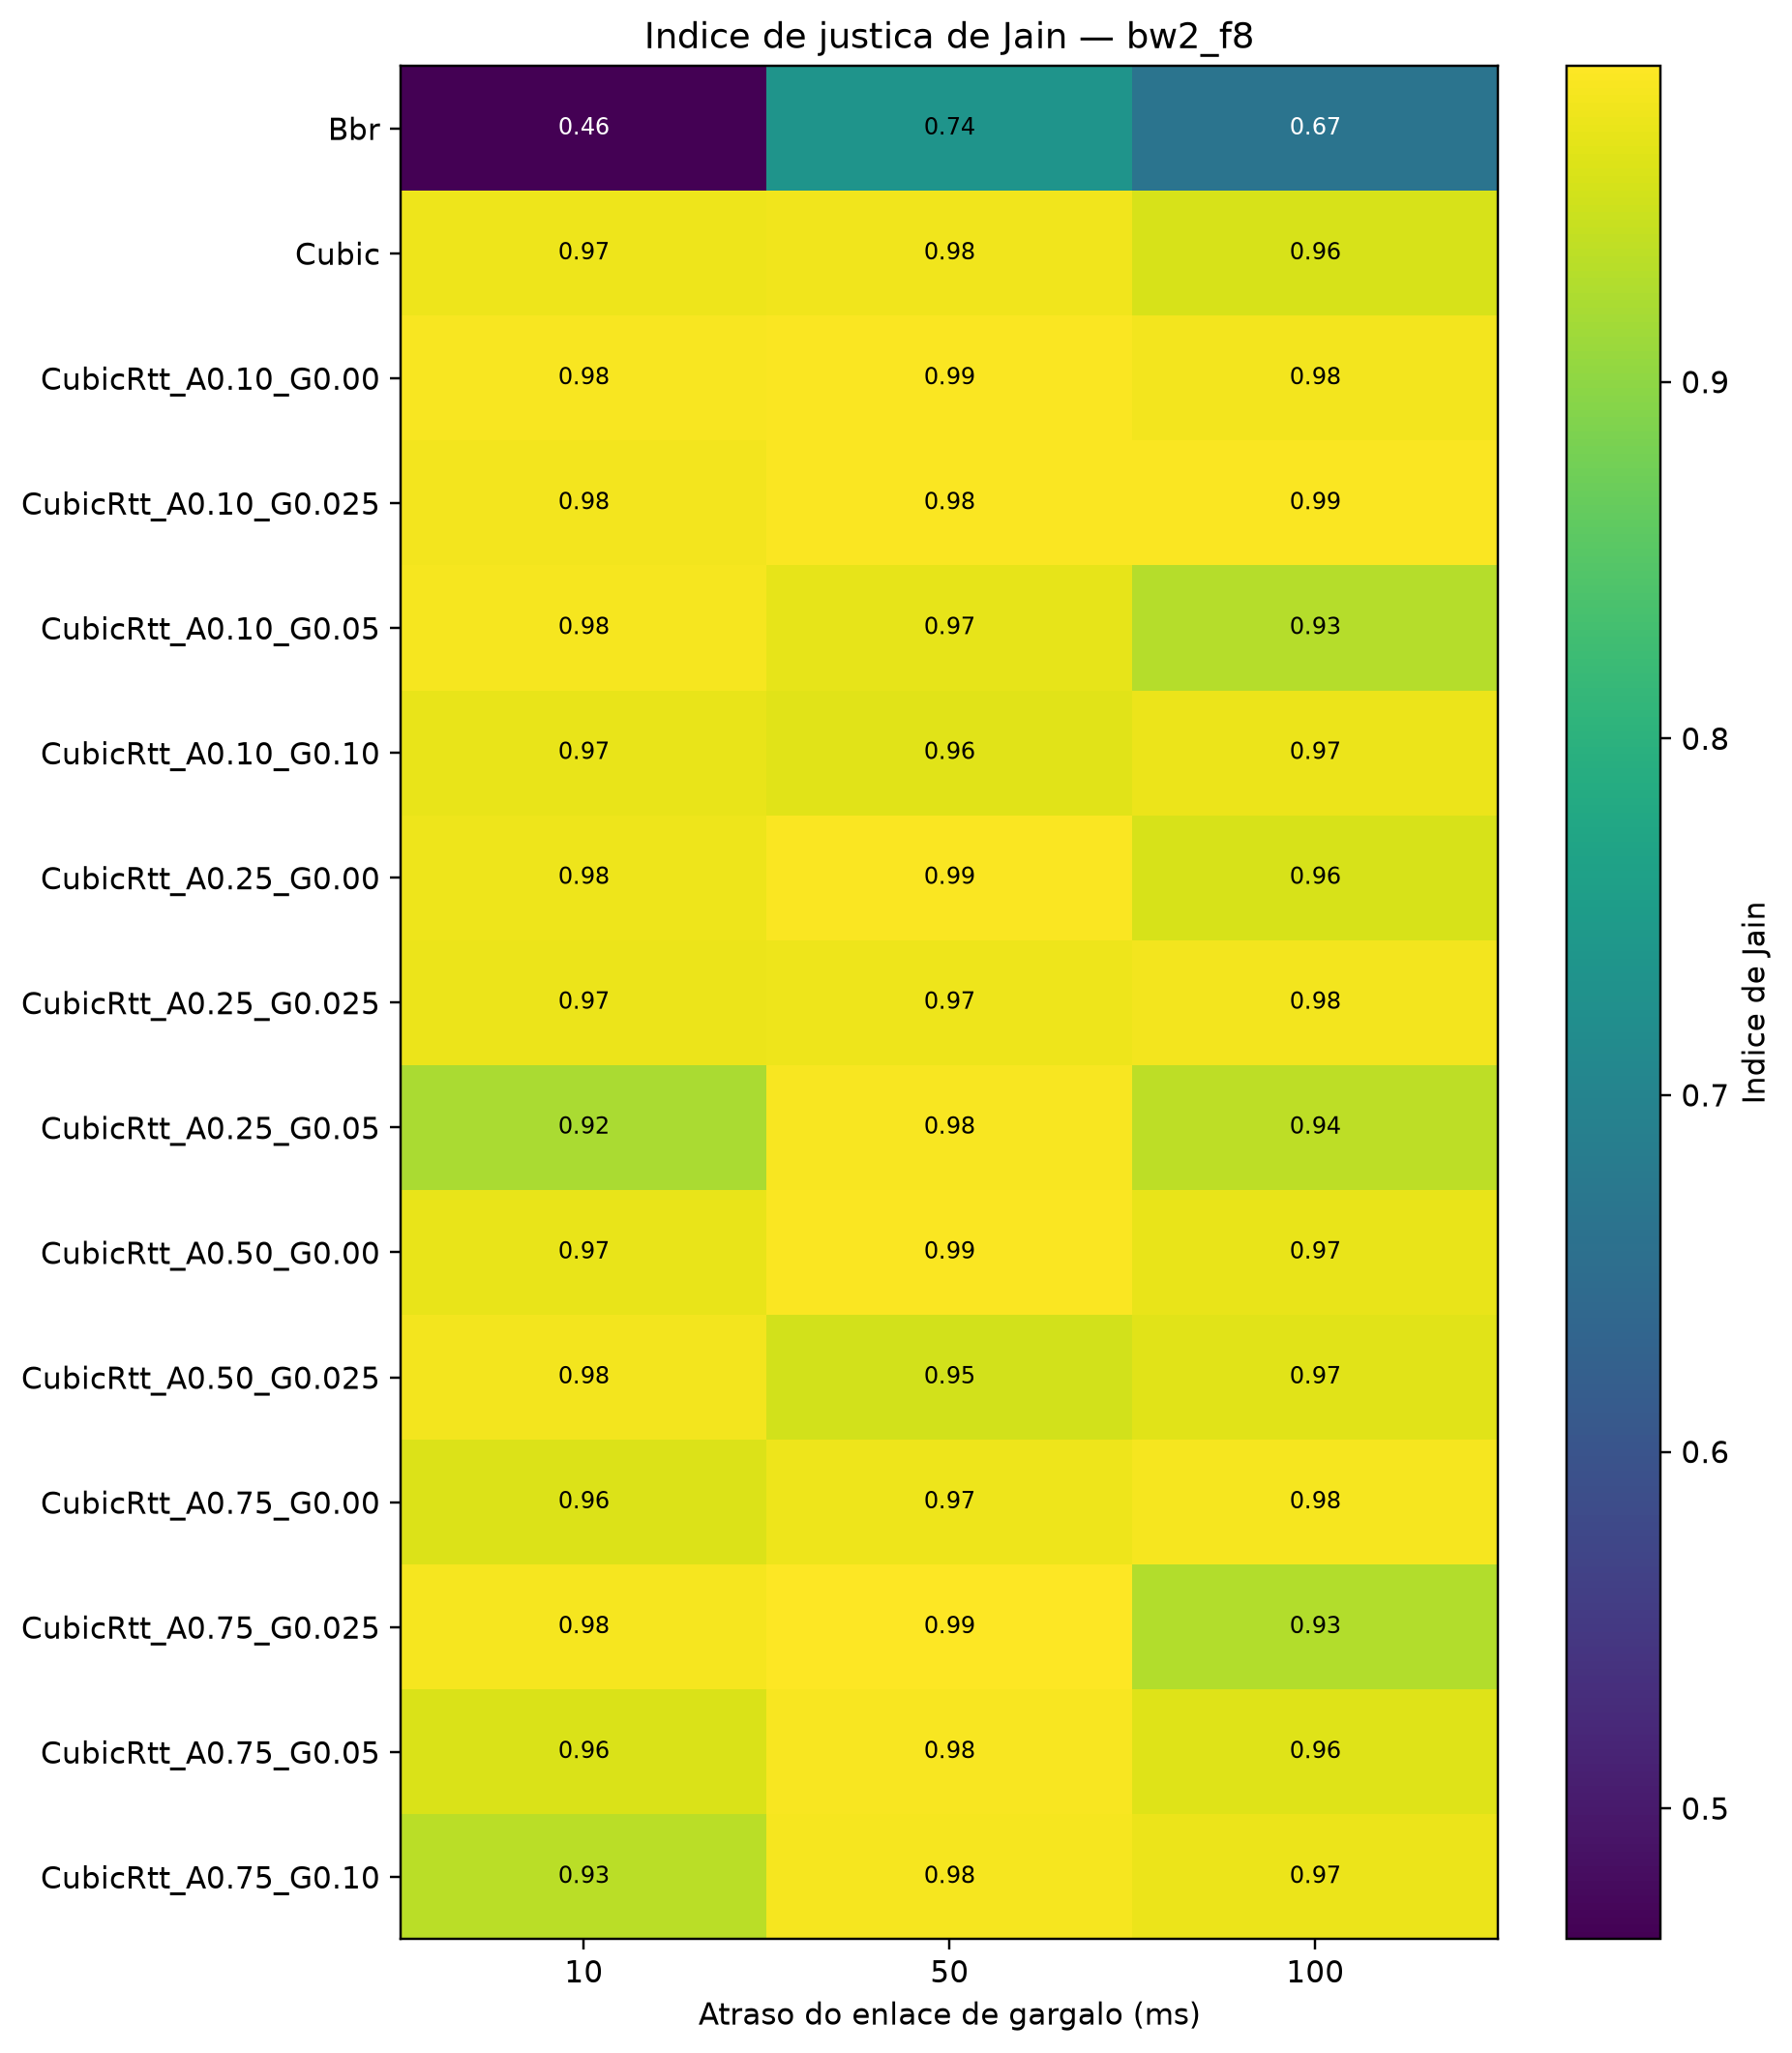
\includegraphics[width=0.88\textwidth]{bw2_f8_jain_fairness.png}
\caption{Índice de Justiça de Jain no cenário \texttt{bw2\_f8}.}
\label{fig:bw2-jain}
\end{figure}
